\chapter{Experiments and Results}
\initial{T}his chapter summarizes the results of the experiments that were performed in the course of this thesis. All results were obtained by employing the Vienna Science Cluster 3 (VSC-3) that was described in Section~\ref{sec:vsc3}. 

First the results of the matrix-matrix multiplication benchmarks are given, both for the sequential and the parallel case. For that, the newly implemented algorithms are analyzed in detail and compared to other algorithms. Afterwards, the performance of a method that falls back on those multiplications is explored, i.e. a dissection of multigrid performance is given.

\section{Sequential Matrix-Matrix Multiplication}

In order to evaluate the performance of different sequential matrix-matrix multiplication implementations, the operation $C = AA$ was carried out on one processor core of the VSC-3. The matrix $A$ here is a matrix that could arise from a Poisson equation when using one of various stencils and a specific grid size. Since there is a row in the matrix for each node of the grid, a $20\times 20 \times 20$ grid for example yields a $20^3 \times 20^3$ matrix.


\subsection{Determining the Best \textit{combined} Implementation}
For the sequential matrix-matrix multiplication, the first thing that had to be evaluated was how the \textit{combined} algorithm should be used. This is the newly implemented algorithm which combines the symbolic and numeric calculations in one step. As described in Chapter~3, the step where a column index is added to an array can be implemented in two ways: One way is to look for the index in the array and add it only if it is not present yet. The other way is to use a flag array that indicates if the index has already been added. 

Both implementations were benchmarked and compared to the \textit{sorted} algorithm, as shown in Fig.~\ref{fig:ex209_insert_append_3d19p}. The three-dimensional 19-point stencil (see next section) was used here and the \textit{combined} algorithm results were normalized to the \textit{sorted} algorithm. 

For this experiment, the \textit{combined} algorithm with \texttt{appendToArray()} (which uses a flag array) delivers a performance that differs less than 5\% from the \textit{sorted} algorithm performance, with a low correlation between grid size and normalized execution time. On the other hand, the fact that an index of the array is searched in each iteration is reflected in the results for the \texttt{insertInArray()} version: This version needs around twice the amount of time that \textit{sorted} needs. Since the \texttt{appendToArray()} version performs so much better, the other version was not used for further benchmarks.

\begin{figure}[tb]
	\centering
	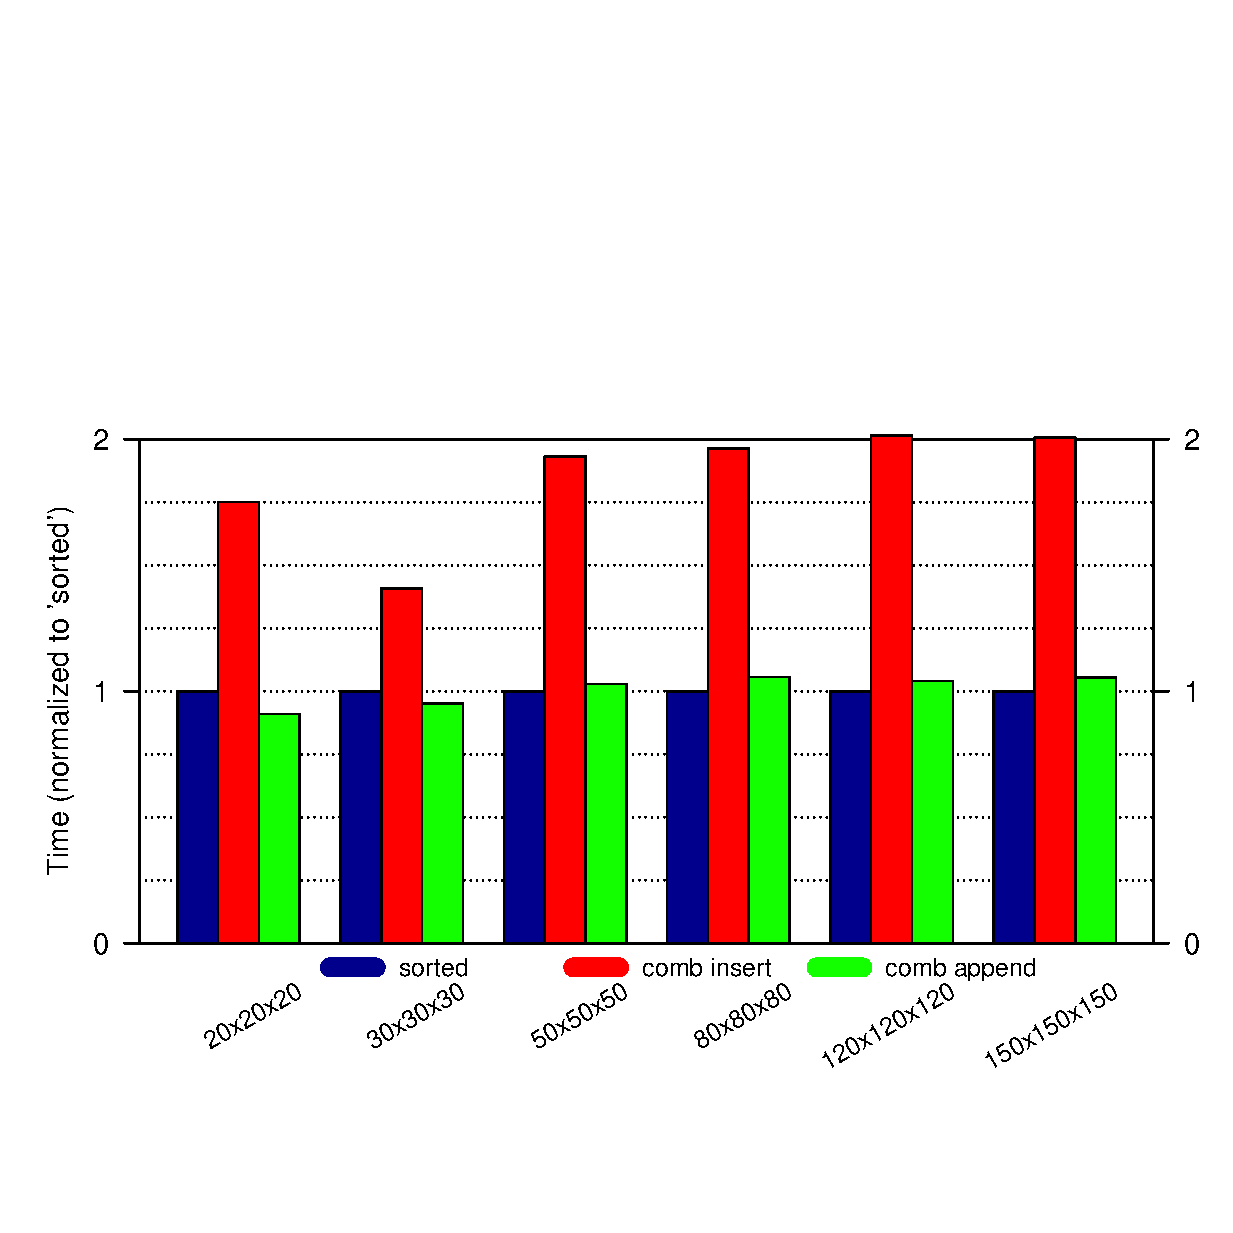
\includegraphics[width=0.99\textwidth, trim={0 2.cm 0 7cm},clip]{seq_insert_append}
	\caption{Sequential MatMatMult(): The two different implementations of the \textit{combined} algorithm (comb insert and comb append) are compared to the \textit{sorted} algorithm of the sequential matrix-matrix multiplication for different grid sizes.} 
	\label{fig:ex209_insert_append_3d19p}
\end{figure}

\subsection{Different Stencils}
Next, the matrix-matrix multiplication was evaluated by using different implementations (which were described in Chapter 3) and different stencils. The number of points in a stencil tells how many points are used for describing an unknown value with a linear combination. In Chapter~2, five points were used to approximate a two-dimensional solution for the Poisson equation. With a higher number of points, the accuracy can be improved (so higher order derivatives are approximated) and three-dimensional simulations can be modeled. However, more points also result in more computational work. Fig.~\ref{fig:stencils} shows different two-dimensional stencils, among them two different 9-point stencils. 

\begin{figure}[tb]
	\centering
	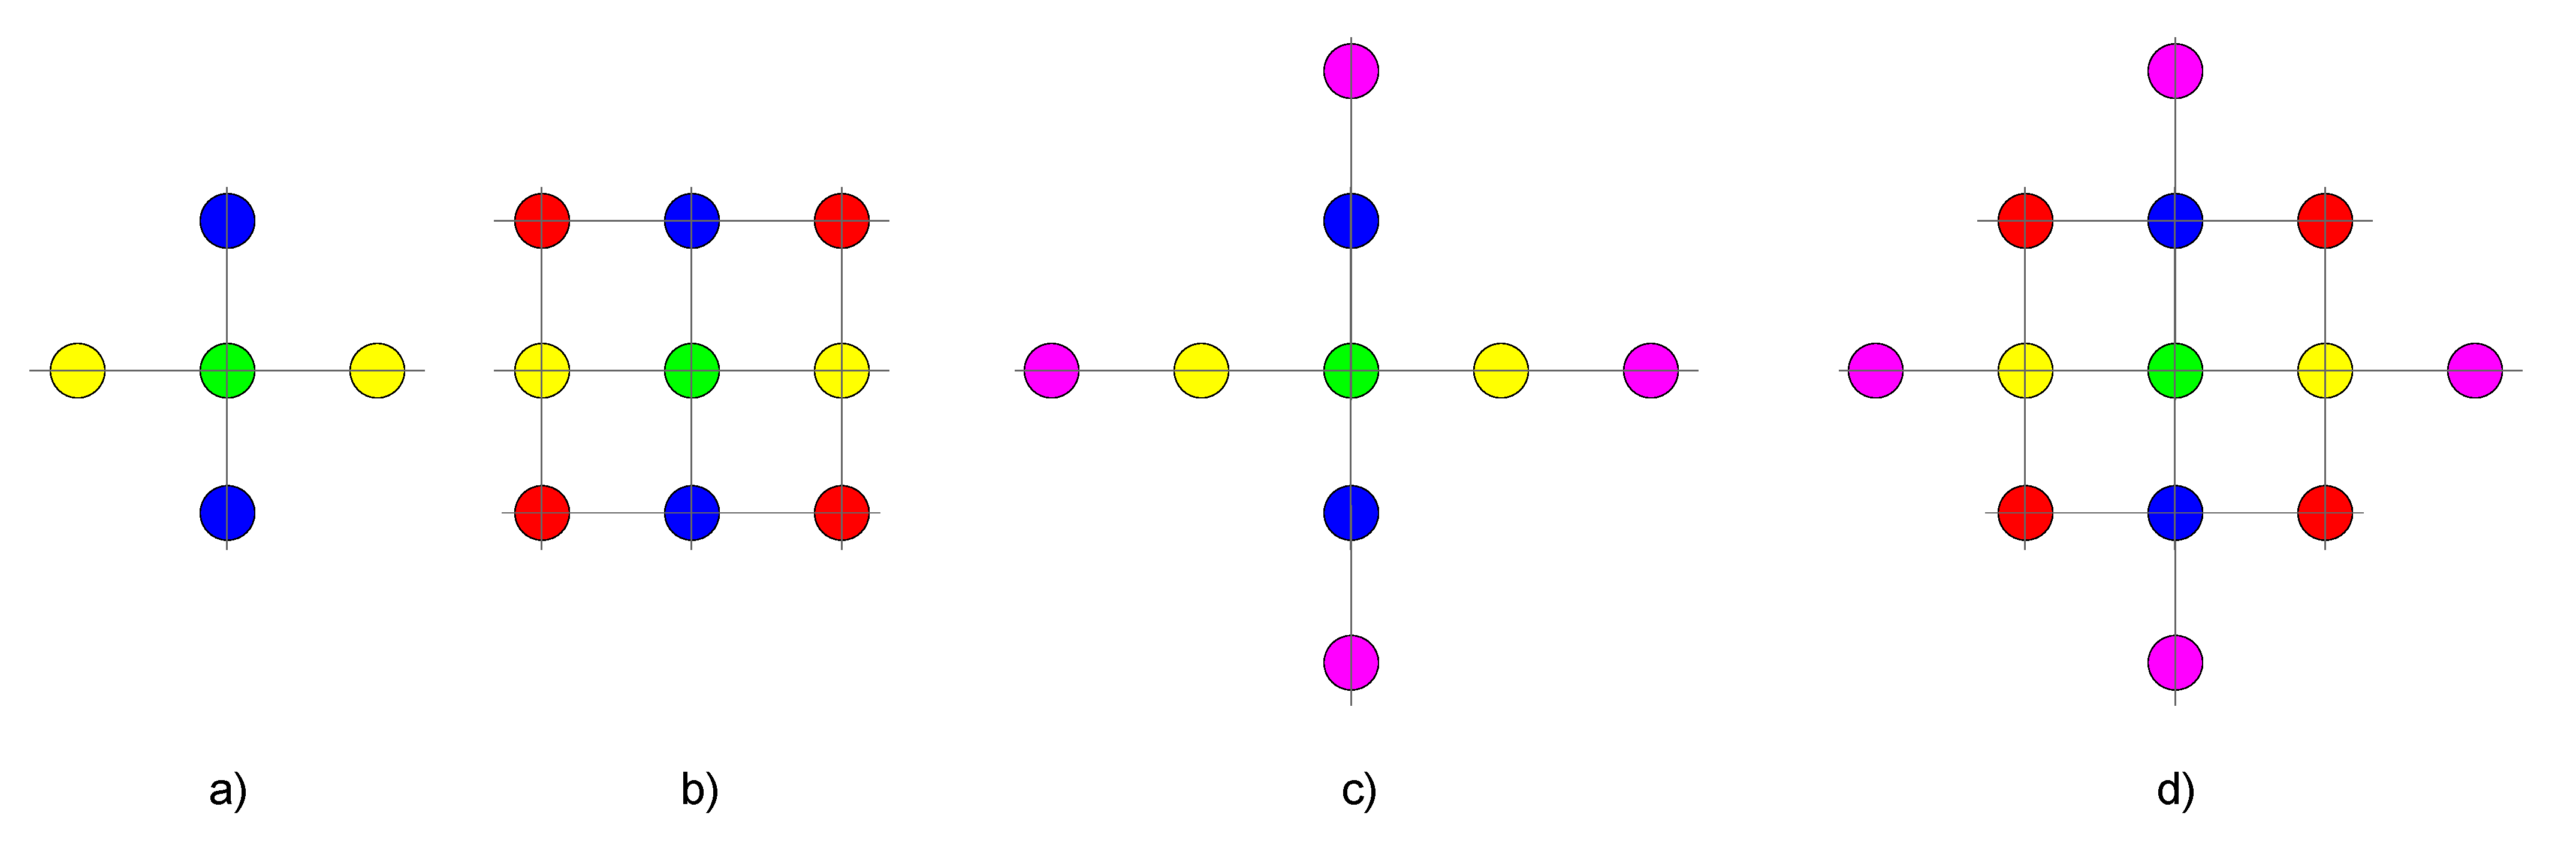
\includegraphics[width=0.99\textwidth, trim={0 0.cm 0 0cm},clip]{stencils}
	\caption{Several two-dimensional stencils. Different colors indicate different absolut values of the coefficients. \textbf{a)} 5-point stencil \textbf{b)} 9-point stencil, \textbf{c)}, another way to form a 9-point stencil, \textbf{d)} 13-point stencil} 
	\label{fig:stencils}
\end{figure}


For these experiments, the grids had a size of $2000 \times 2000$ for the 2d stencils and $100\times 100 \times 100$ for the 3d stencils. As can be seen in Fig.~\ref{fig:ex209_R}, the newly implemented \textit{combined} algorithm (with \texttt{appendToArray()} function) performs quite well for all stencils. It is faster than the very similar \textit{sorted}-algorithm for most stencils, and it is the fastest algorithm for big stencils, i.e. for matrices that are not extremely sparse. The \textit{combined} algorithm is very often around 10-20\% faster than the \textit{sorted} algorithm, and only for small stencils, the \textit{rowmerge} algorithms perform better (up to 25\% faster). Except for the \textit{scalable} and the \textit{btheap} algorithm, the implementations show acceptable results. What is remarkable here is that the normalized execution time of the \textit{scalable} algorithm increases with the size of the stencil.

% ex 209
\begin{figure}[tb]
	\centering
	\hspace*{-10mm}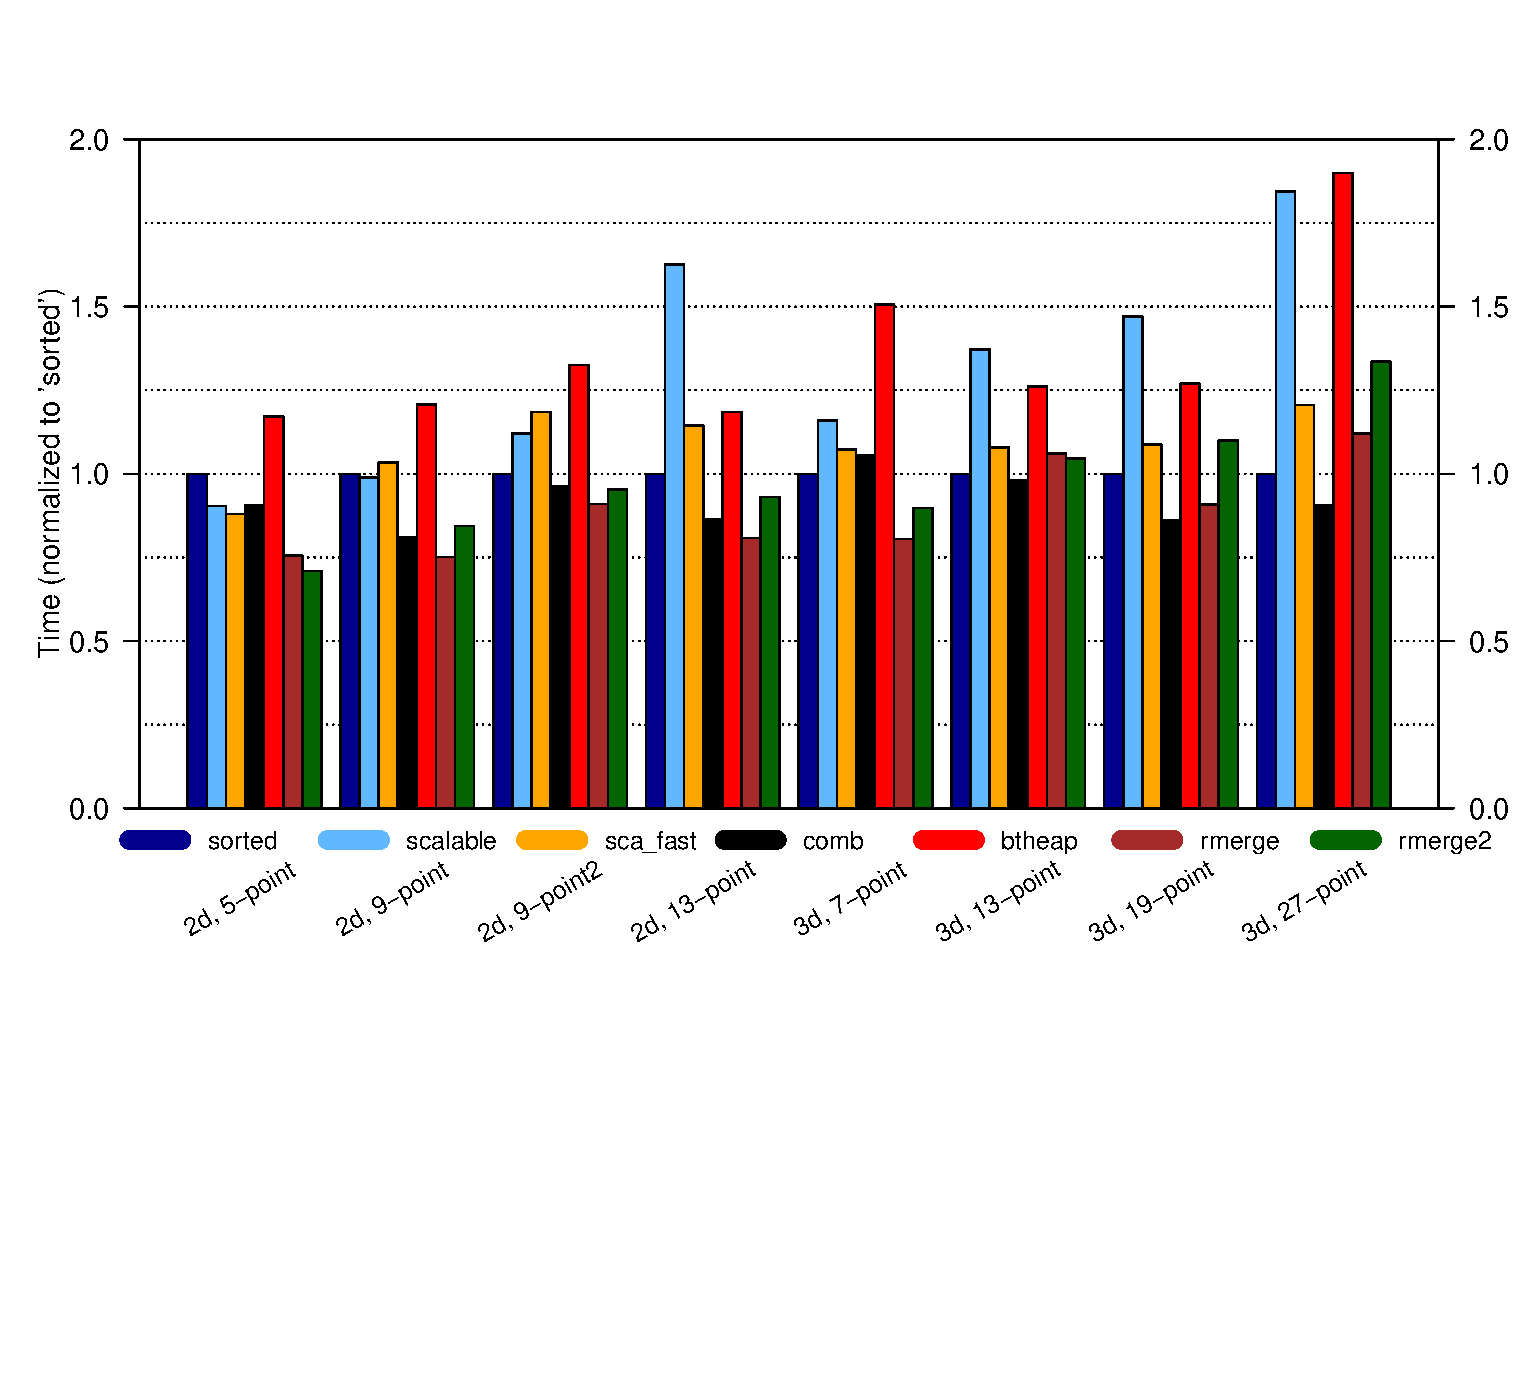
\includegraphics[width=1.1\textwidth, trim={0 7.cm 0 1.6cm},clip]{petsc-matmatmult}
	\caption{Sequential matrix matrix multiplication for different stencils and implementations.  } 
	\label{fig:ex209_R}
\end{figure}

\subsection{Different Grid Sizes}

In the previous experiment, the grid size was fixed and the results of different stencils were shown. Now, the performance is evaluated for a certain stencil and different grid sizes. 

First, we take a look at the performance when using the small 2d, 5-point stencil (see Fig.~\ref{fig:seq2d5point}). This means the matrix $A$ has only 5 non-zeros per row (out of $\approx 67$ million entries per row for the largest tested grid). As can be seen, the \textit{rowmerge2} algorithm suits this problem best, needing only half of the time the \textit{sorted} algorithm needs. The \textit{combined} algorithm performs moderately and is slightly better than the \textit{sorted} algorithm. In general, we observe that the ranking of the different algorithms is more or less the same for small and large grids and also the execution time ratios do not change very much. Only the \textit{btheap} algorithm shows big variations in performance.

\begin{figure}[tbp]
	\centering
	\hspace*{-7mm}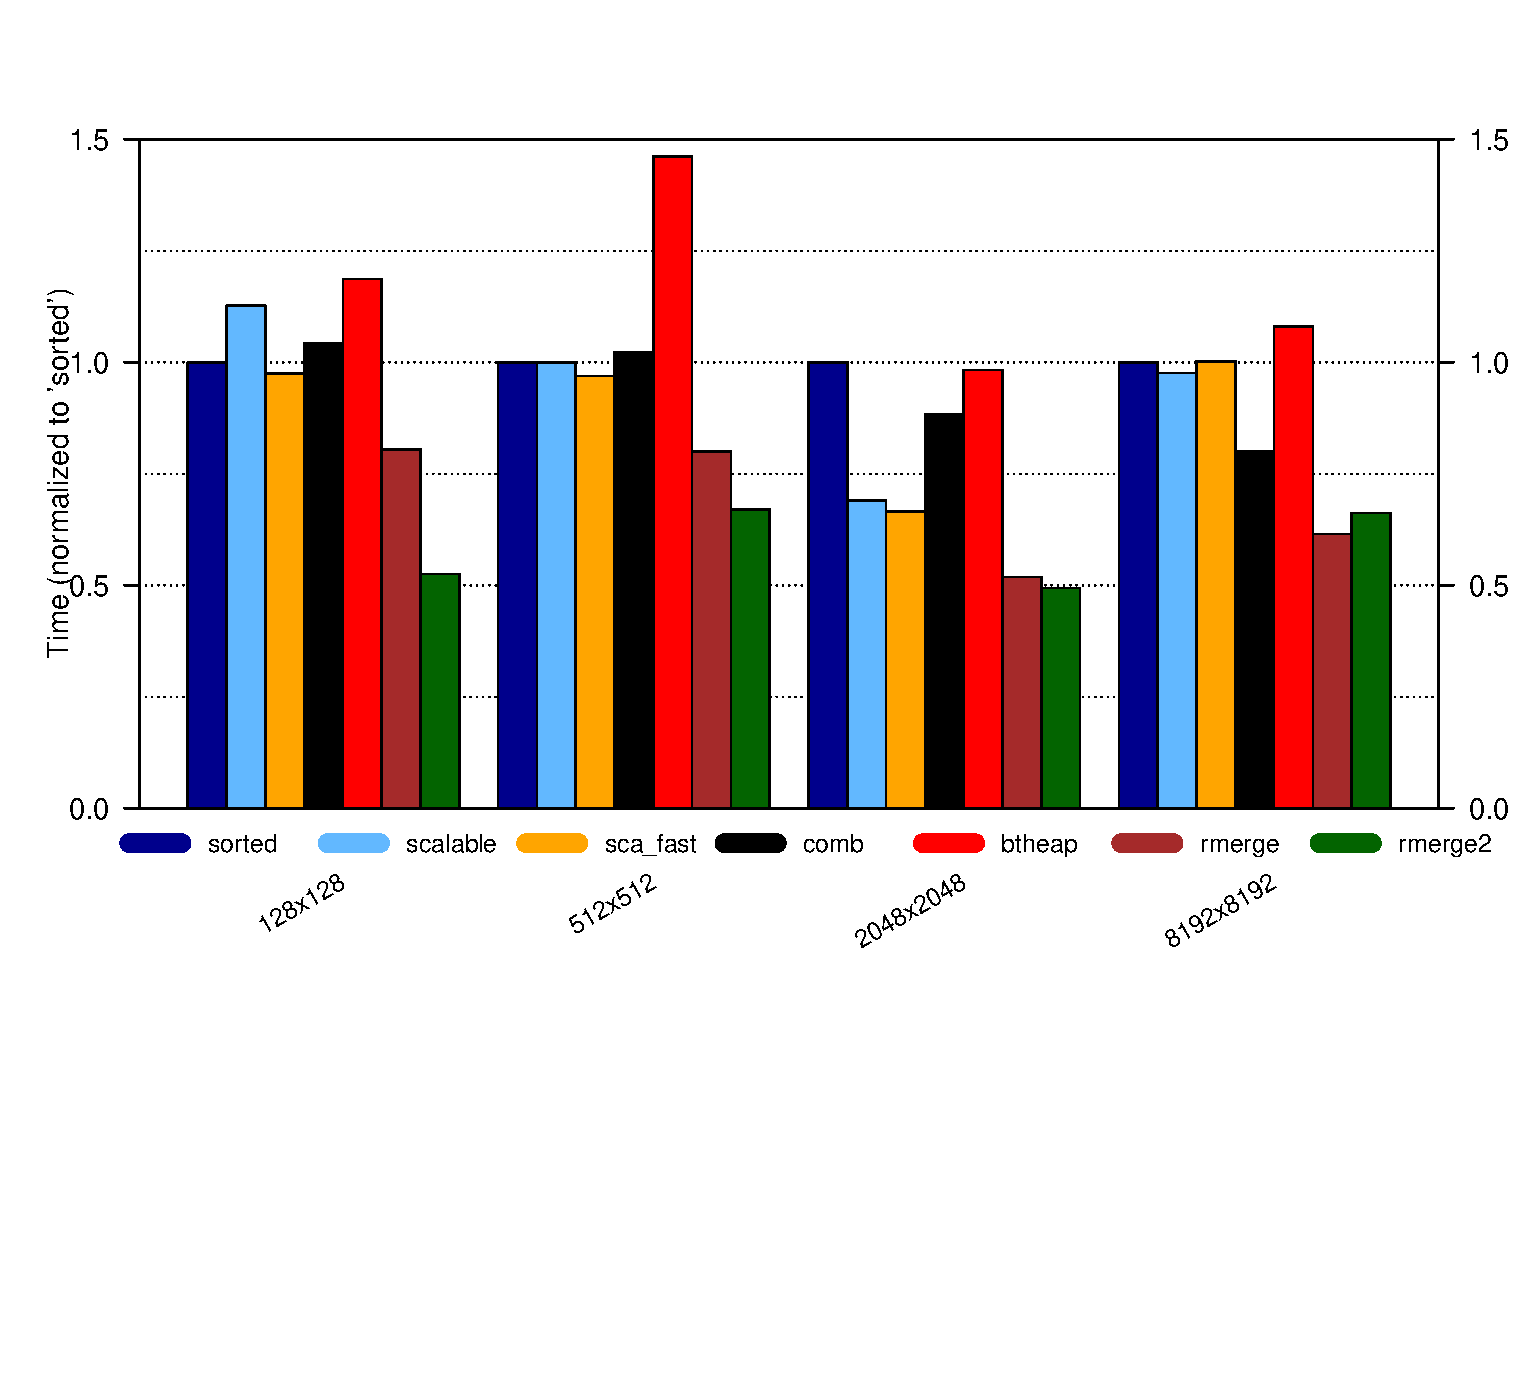
\includegraphics[width=1.05\textwidth, trim={0 6.9cm 0 1cm},clip]{seq_2d5point}
	\caption{2d, 5-point stencil: Matrix multiplication with this stencil performed on matrices obtained from different grids.} 
	\label{fig:seq2d5point}
\end{figure}

The same evaluation is now done with a medium-sized stencil, the 2d, 13-point stencil (see Fig.~\ref{fig:seq2d13point}). This means there are now 13 non-zeros per row (out of 4 million entries per row for the largest tested grid). Now the situation changed quite a lot: The two \textit{rowmerge} algorithms are not always the best choice any more and especially the \textit{scalable} algorithm, which delivered a quite good performance before, now performs very poor: For all tested grids, it is about 1.7 times slower than the \textit{sorted} algorithm. Now the differences between the \textit{sorted}, the \textit{combined} and the \textit{rowmerge} algorithms are low (less than 10\%), so any of them is a reasonable choice for this stencil. Only for the $1000 \times 1000$ grid, the \textit{combined} algorithm is much faster (ca. 10\%) than the \textit{sorted} algorithm.

\begin{figure}[tbp]
	\centering
	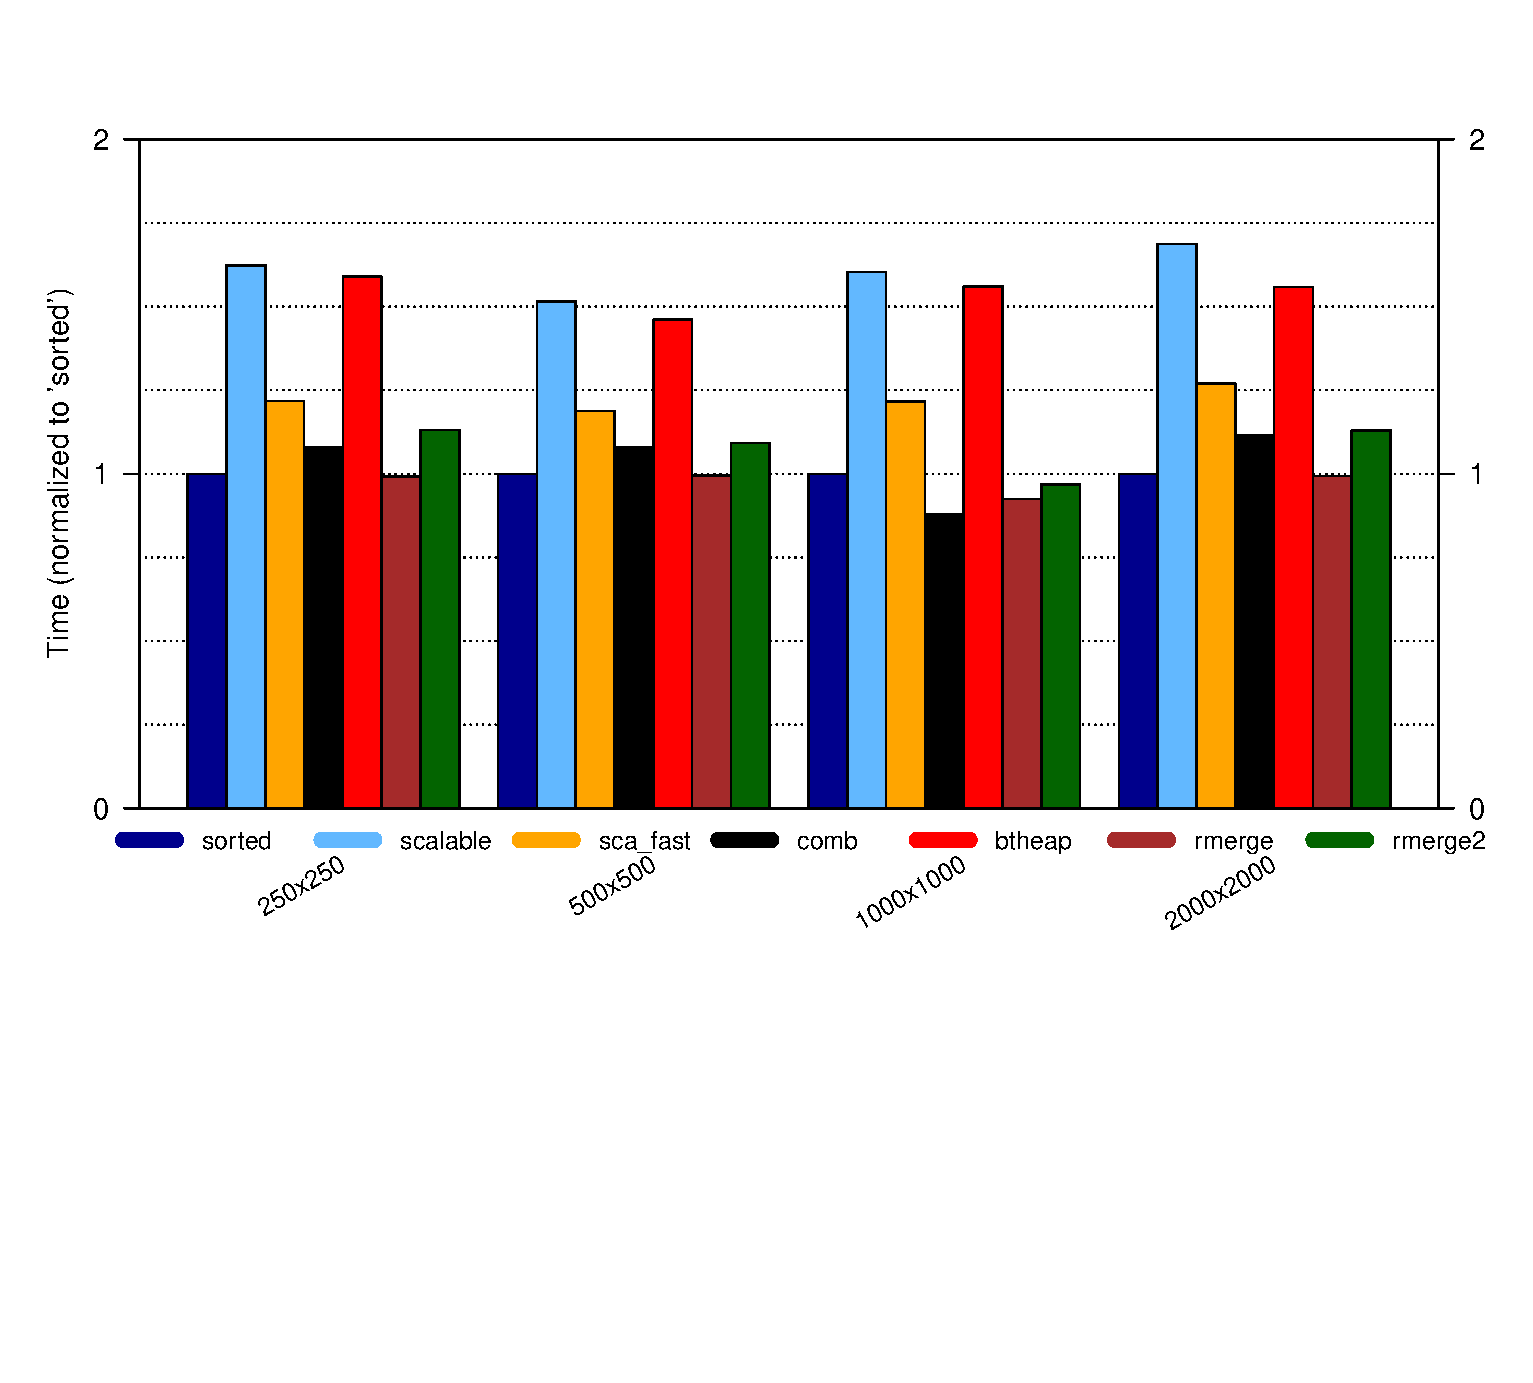
\includegraphics[width=1.1\textwidth, trim={0 7.3cm 0 1cm},clip]{seq_2d13point}
	\caption{2d, 13-point stencil} 
	\label{fig:seq2d13point}
\end{figure}


When using the big 3d, 27-point stencil, there are 27 non-zeros per row (out of 1.7 million entries per row for the largest tested grid). Now the trend of the \textit{scalable} and the \textit{rowmerge} algorithms continues (see Fig.~\ref{fig:seq3d27point}). The \textit{rowmerge} algorithms now need around 25\% more time than the \textit{sorted} algorithm, while the execution time of the \textit{scalable} algorithm increases with the grid size. This behaviour reaches a point where the scalable algorithm needs 2.25 times longer the \textit{sorted} algorithm. This shows that the \textit{scalable} algorithm is only memory-wise scalable, but not performance-wise. The \textit{combined} algorithm, proves to be the fastest algorithm for such a big grid, with a performance that is very similar to the \textit{sorted} performance. 

\begin{figure}[tbp]
	\centering
	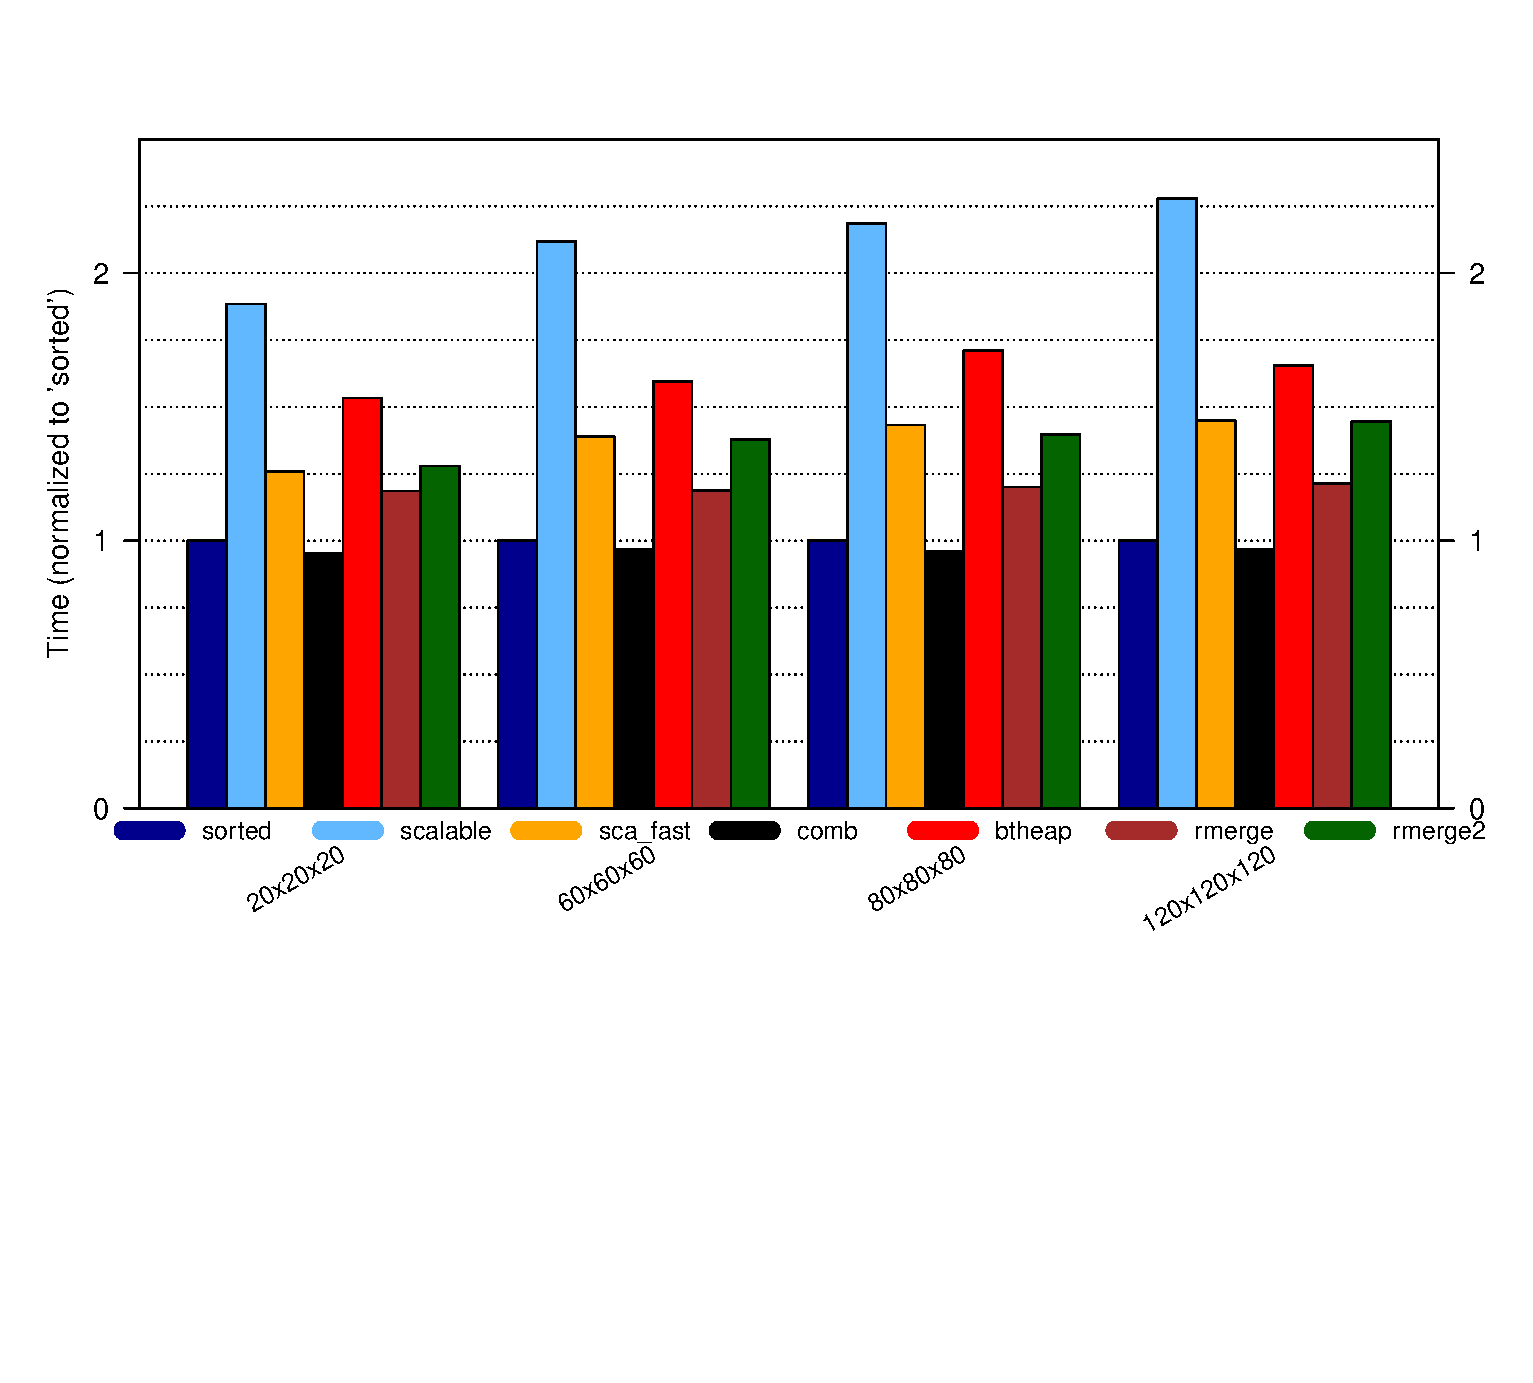
\includegraphics[width=1.05\textwidth, trim={0 7.3cm 0 1cm},clip]{seq_3d27point}
	\caption{3d, 27-point stencil} 
	\label{fig:seq3d27point}
\end{figure}

This section is concluded by noting that the selected stencil has a much bigger impact on the ranking of the algorithms than the grid size. For small stencils, the \textit{rowmerge2} algorithm proves to be the best choice, as it needs only half the time the \textit{sorted} algorithm needs for some test cases. On the other hand, it performs quite poor (up to 40\% slower than \textit{sorted}) for some big stencils and most often, \textit{rowmerge} is around 5-10\% faster than \textit{rowmerge2}. The newly implemented \textit{combined} algorithm is a good choice for most stencils with a performance that is slightly better than the \textit{sorted} performance for many cases. This is only topped by the \textit{rowmerge} algorithms for small stencils (especially \textit{rowmerge} rather than \textit{rowmerge2}). The \textit{bt heap} and the \textit{scalable} algorithms perform moderately for small stencils, but are not suitable for big stencils.

\subsection{Time Ratio: Symbolic Calculation to Total Time}
As discussed in Chapter~3, the matrix multiplication comprises two stages, a symbolic stage and a numeric stage. In order to see which stage should be further optimized, the time spent on each stage was measured. Fig.~\ref{fig:seqsymnum} shows results for small, medium and big stencils, and for small and big grids. 

Since there is no separation of different stages for the \textit{combined} algorithm, it is illustrated as 100\% for the symbolic part. What is very interesting in these results is that the time ratios for the stages depend only very little on the grid size and the stencil. The only big variation can be seen for the \textit{scalable\_fast} algorithm, where the ratio for the symbolic stage ranges from around 50\% for medium and big stencils to 80\% for small stencils. For the two \textit{rowmerge} algorithms, a positive correlation between the stencil size and the time ratio for the symbolic stage can be observed. Except for the two \textit{scalable} and the \textit{combined} algorithm, the symbolic stage takes around 80\% of the time. In conclusion, this data tells us that the numeric stage of the \textit{scalable\_fast} algorithm and the symbolic stage of the other algorithms are attractive for optimization.

\begin{figure}[tbp]
	\centering
	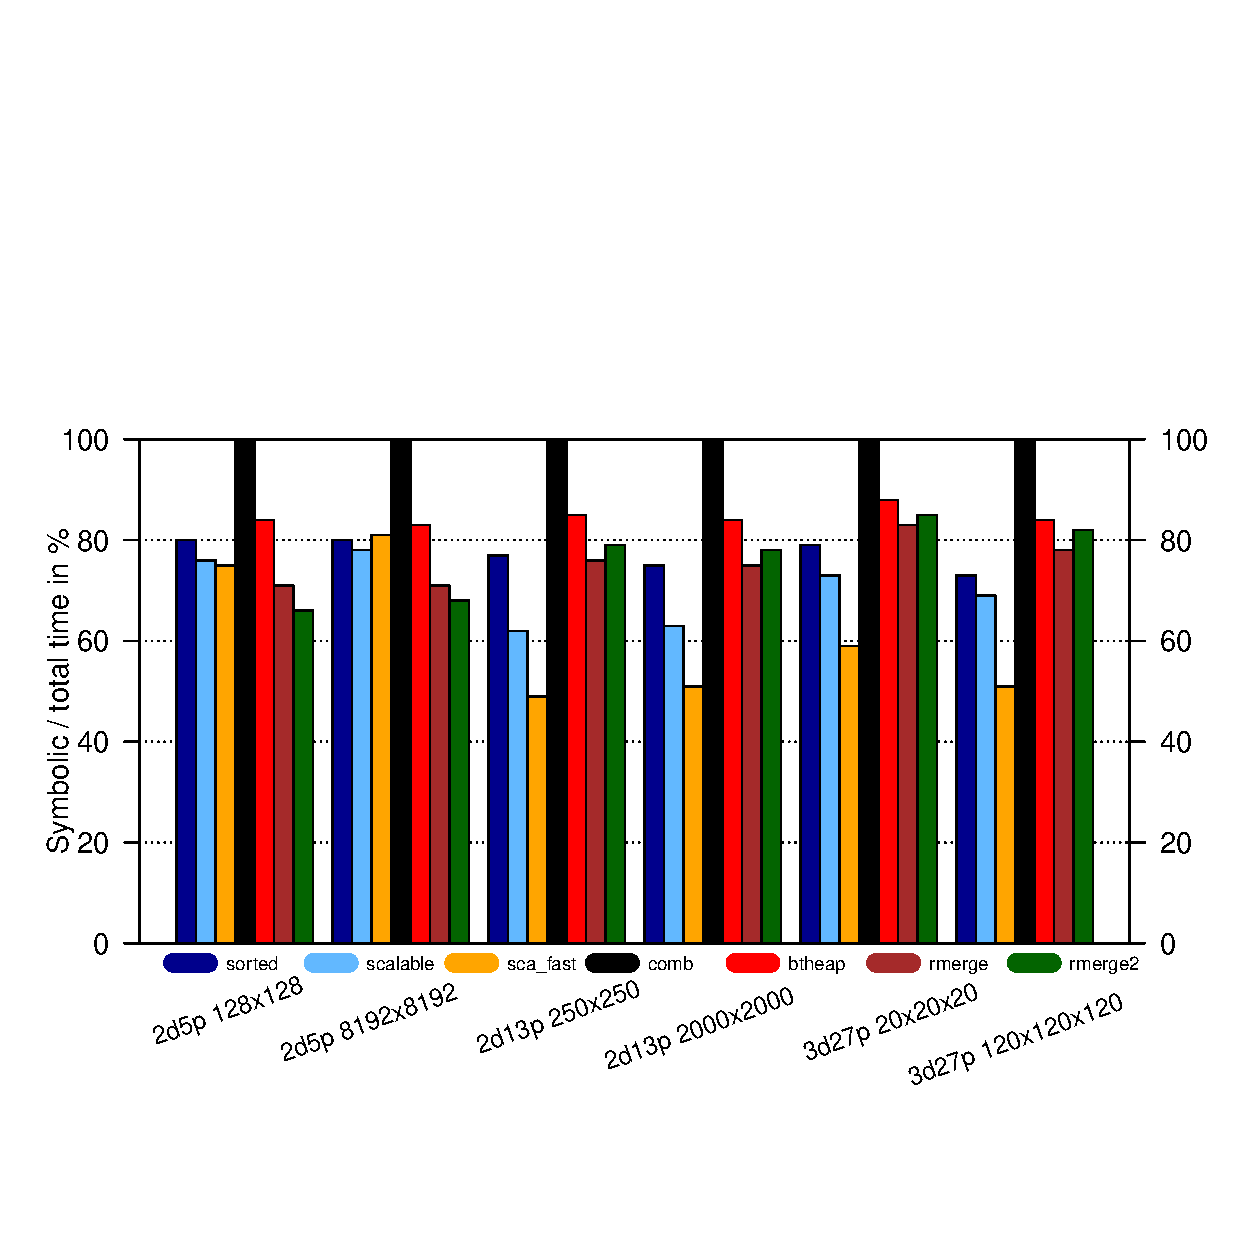
\includegraphics[width=1.05\textwidth, trim={0 2.cm 0 6cm},clip]{seq_symnum}
	\caption{Percentage of the symbolic stage of the matrix multiplication of the total execution time. The rest to 100\% is spent on the numeric stage. For the combined algorithm, everything is combined in one stage.} 
	\label{fig:seqsymnum}
\end{figure}


\section{The \textit{PtAP} Multiplication}
Another operation that was evaluated is the sparse matrix product $C = P^T A P$ (Galerkin product) that was introduced in Section~\ref{sec:PtAP}. This can either be computed directly with a specialized algorithm, or by performing one of the naive approaches $C = (P^T A) P$ or $C = P^T (A P)$. The results can be seen in Fig.~\ref{fig:ex2_ptap}. Since the results are so similar to each other, a high accuracy was necessary here, which was obtained by taking the median value of 41 measurements.

As can be seen, the direct method is slightly faster than the two other methods for all grid sizes. 	Since the performance differences are so small, it was decided that no further optimizations on this algorithm are to be done for now.

\begin{figure}[tbp]
	\centering
	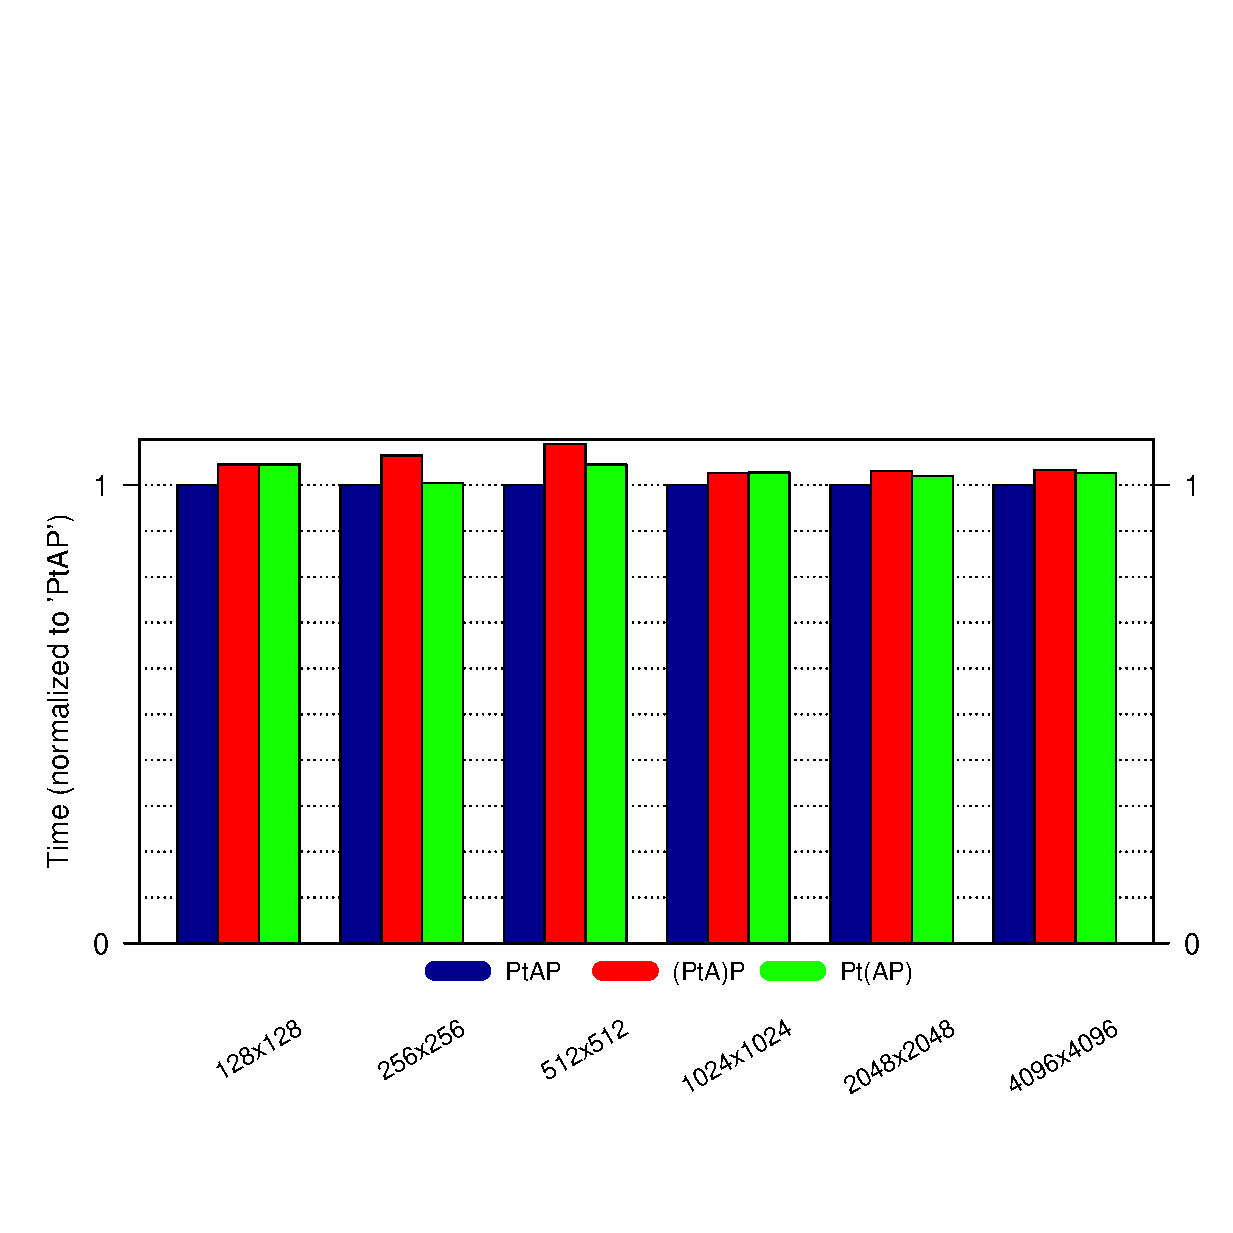
\includegraphics[width=0.99\textwidth,  trim={0 2.cm 0 6cm},clip]{ex2_PtAP}
	\caption{Normalized time for different implementation of the Galerkin product.} 
	\label{fig:ex2_ptap}
\end{figure}

\section{Parallel Matrix-Matrix Multiplication}
For the parallel matrix-matrix multiplication, there are two existing implementations, a scalable one and a non-scalable one. Similar to the sequential algorithm, the array with the array indices that refer to non-zero entries is of variable size for the scalable algorithm and of fixed size (only dependent on the number of columns in the matrix) for the non-scalable algorithm. Since the matrices are divided among the processes in a way where complete rows are  associated with a process, this fixed sized array for the non-scalable implementation has a length that is equal to the number of columns in the matrix $B$. 

\subsection{A Basis for a New Implementation}
In order to see if the new implementation in this thesis (see Section~\ref{sec:seq_mpi}) should be based on a scalable or non-scalable approach, their performance had to be evaluated. Fig.~\ref{fig:scalable} shows the results of a matrix-matrix multiplication with 8 processes for a 3d, 27-point stencil and different local grid sizes. For the smallest tested grid, the \textit{scalable} algorithm is already ca. 70\% slower than the non-scalable algorithm. With bigger grids, this difference increases very quickly: For the biggest tested grid, the \textit{scalable} version is already 30 times slower than the \textit{nonscalable} implementation. This biggest tested grid of local size $60 \times 60 \times 60$ (this corresponds to a global size of $120\times 120 \times 120$ for 8 processes) is still much smaller than other grids that were tested with the \textit{nonscalable} algorithm. However, even with data limited to small and medium sized grids, it is obvious that the \textit{scalable} algorithm is not a reasonable choice for big systems. 

The reason for this lack in performance for the \textit{scalable} algorithm lies in the fact that new memory has to be allocated for new column indices very often, which is extremely expensive. Since the \textit{nonscalable} implementation performs so much better, the new implementation is based on a non-scalable approach. 

\begin{figure}[tbp]
	\centering
	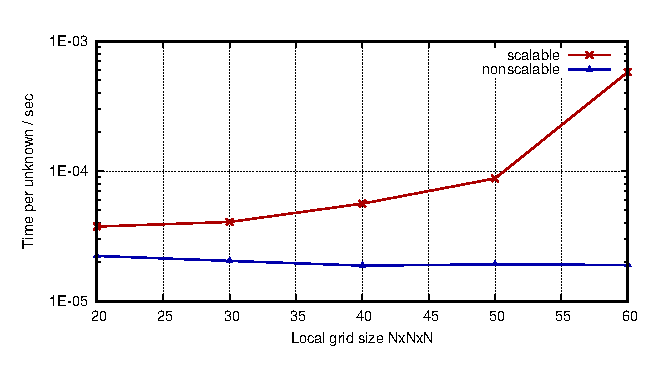
\includegraphics[width=1\textwidth]{scalable}
	\caption{The \textit{scalable} algorithm proves to be very slow, even for medium sized grids. In this test, it is up to 30 times slower than the \textit{non-scalable} implementation.} 
	\label{fig:scalable}
\end{figure}

\subsection{Comparison: Non-Scalable vs Sequential MPI}
The existing \textit{nonscalable} algorithm (see Section~\ref{sec:existing_impl}) was compared to the new \textit{sequential MPI} algorithm (see Section~\ref{sec:seq_mpi}), which uses sequential matrix multiplication routines on many MPI ranks at the same time. This was tested for 2d and 3d stencils, and for different grid sizes.

\subsubsection*{2d stencils}
Fig.~\ref{fig:mat_ex_test_ex2_times_2d} shows the results for different 2d stencils and for 32 processes (4 nodes with 8 processes each). 

It can be seen that the time per unknown remains quite constant for large grids. Only for small grids, considerably more time is needed because latencies oppress the performance.


For the very small 2d, 5-point stencil the \textit{nonscalable} version is quicker than the \textit{seq mpi} version for all tested grid sizes. The absolute time difference between the two versions and the time per unknown are both remarkably constant. 

With the 2d, 9-point stencil the behaviour of the two implementations is very similar, but due to more elements in the matrix (more connections between grid points), the time per unknown is bigger. Also, the difference between the two implementations is smaller now (less than 5\% for big grids). 

For the 2d, 13-point stencil and big grids, the \textit{seq mpi} algorithm finally shows slightly better results than the other implementation. However, for small grids, this algorithm is still slower than the \textit{nonscalable} algorithm. 

\begin{figure}[tbp]
	\centering
	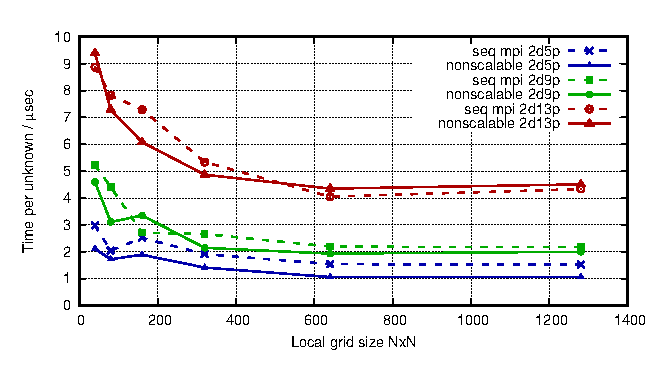
\includegraphics[width=1\textwidth]{times_2d}
	\caption{} 
	\label{fig:mat_ex_test_ex2_times_2d}
\end{figure}

\subsubsection*{3d stencils}
A local grid size of up to $100 \times 100 \times 100$ (which corresponds to $317 \times 317 \times 317$ in global size) with 32 MPI-ranks was used to evaluate the performance of the two implementations.  Fig.~\ref{fig:mat_ex_test_ex2_times_3dsmall} shows the results for small grids. For both stencils, we observe that for small grids, the time per unknown is almost 3 times higher than for the big grids. Again, this is due to latencies that take a big share of the total time when dealing with small grids.

For the 3d, 7-point stencil and for both implementations, the time per unknown changes only very little for grids with $N \gtrapprox 40$ (around 2$\mu  s$ per unknown for the \textit{nonscalable} implementation). The \textit{sequential MPI} implementation is around 25\% slower. For the 3d, 13-point stencil, the difference between the two implementations is very little with no clearly faster version. 


\begin{figure}[tbp]
	\centering
	\vspace*{-2.5mm}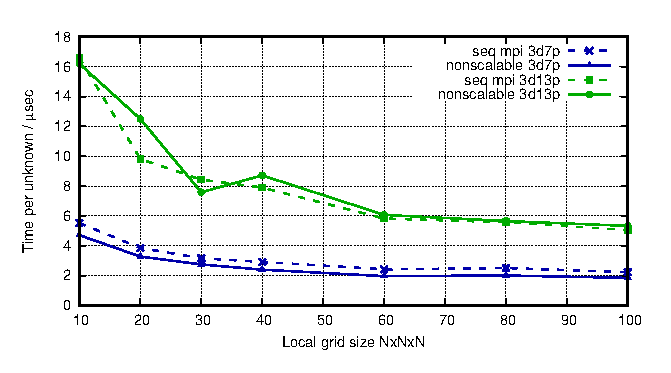
\includegraphics[width=1\textwidth]{times_3dsmall}
	\caption{Parallel matrix multiplication for small 3d stencils. } 
	\label{fig:mat_ex_test_ex2_times_3dsmall}
\end{figure}

Fig.~\ref{fig:mat_ex_test_ex2_times_3dlarge} shows the time per unknown for big 3d stencils. Now the time per unknown does not change much for grids with $N > 30$. For these big grids, the \textit{sequential MPI} implementation is clearly faster: With the 3d, 27-point stencil, the \textit{nonscalable} implementation needs around 50\% more time than the \textit{seq mpi} implementation. 

In conclusion, we note that the \textit{nonscalable} implementation is usually faster for both small and big grids, if the used stencil is small, i.e. if the stencil has less than 13 points. This is true for both 2d and 3d stencils. For 13-point stencils, there is no clear winner, but with more than 13 points in a stencil, the new \textit{sequential MPI} performs up to 50\% better than the existing \textit{nonscalable} implementation.

\begin{figure}[tbp]
	\centering
	\vspace*{-2.5mm}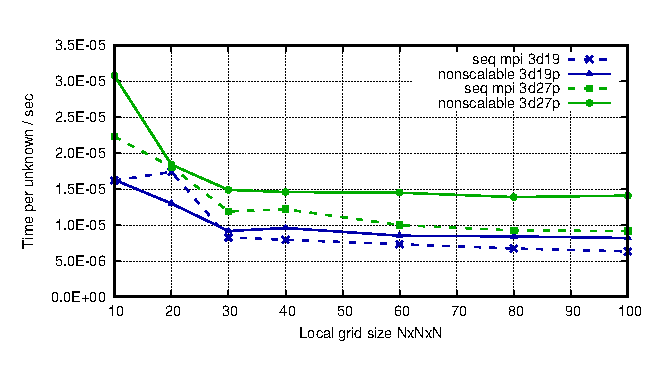
\includegraphics[width=1\textwidth]{times_3dlarge}
	\caption{Parallel matrix multiplication for large 3d stencils.} 
	\label{fig:mat_ex_test_ex2_times_3dlarge}
\end{figure}

\subsection{Time Division of the \textit{Sequential MPI} Implementation}

Next the time consumption of different parts of the \textit{sequential MPI} implementation is analyzed. For that, the algorithm was divided into 10 essential sections, which add up to 100\% of the symbolic calculation:

\begin{itemize}
\item Memory allocations: This includes malloc(), calloc(), PetscNew() functions and other functions for creating arrays.
\item Get \textit{B} rows: This is the step where the non-local rows of $B$ that are needed for the calculation, are being retrieved from other processors.
\item Correct indices: Here the column index of the result of $A_{\textrm{loc, diag}} B_{\textrm{loc, diag}}$ are converted from local indices to global indices.
\item Set \texttt{dnz} and \texttt{onz}: The arrays \texttt{dnz} and \texttt{onz} store information about the number of non-zero entries in the diagonal and offdiagonal part of each row. This information is calculated in this step. 
\item Merge: In this step, the result rows of the multiplications $A_{\textrm{loc, diag~}} B_{\textrm{loc, diag}}$,   \\$A_{\textrm{loc, diag~}} B_{\textrm{loc, off}}$ and $A_{\textrm{loc, off~}} B_{\textrm{nonloc}}$ are merged into one final result row.
\item Preallocations: The diagonal and offdiagonal parts of each row have to be preallocated with information from \texttt{dnz} and \texttt{onz} in order to quickly create a matrix.
\item Set matrix values (matSetVal): Once the matrix columns are finally computed, they have to be copied to the matrix. This is done here.
\item Mat1: The symbolic multiplication $A_{\textrm{loc, diag~}} B_{\textrm{loc, diag}}$.
\item Mat2: The symbolic multiplication $A_{\textrm{loc, diag~}} B_{\textrm{loc, off}}$.
\item Mat3: The symbolic multiplication $A_{\textrm{loc, off~}} B_{\textrm{nonloc}}$.
\end{itemize}

The percentages of each step are measured for different matrix sizes, stencils and numbers of processes and the results are given in the following.

\subsubsection*{10240 $\times$ 10240, 256 cores}
Fig.~\ref{fig:pie_256_10240} shows the results for a $10240 \times 10240$ grid with a 2d, 13-point stencil. The multiplication was performed on 16 nodes with 16 cores each, resulting in 256 cores. Rather surprisingly, only a third of the total time is spent on actual matrix multiplications. Since most matrix elements lie in the diagonal of the matrix, the multiplication $A_{\textrm{loc, diag}}~B_{\textrm{loc, diag}}$ needs much more time than the multiplications dealing with the few non-local elements. 

\begin{figure}[tbp]
	\centering
	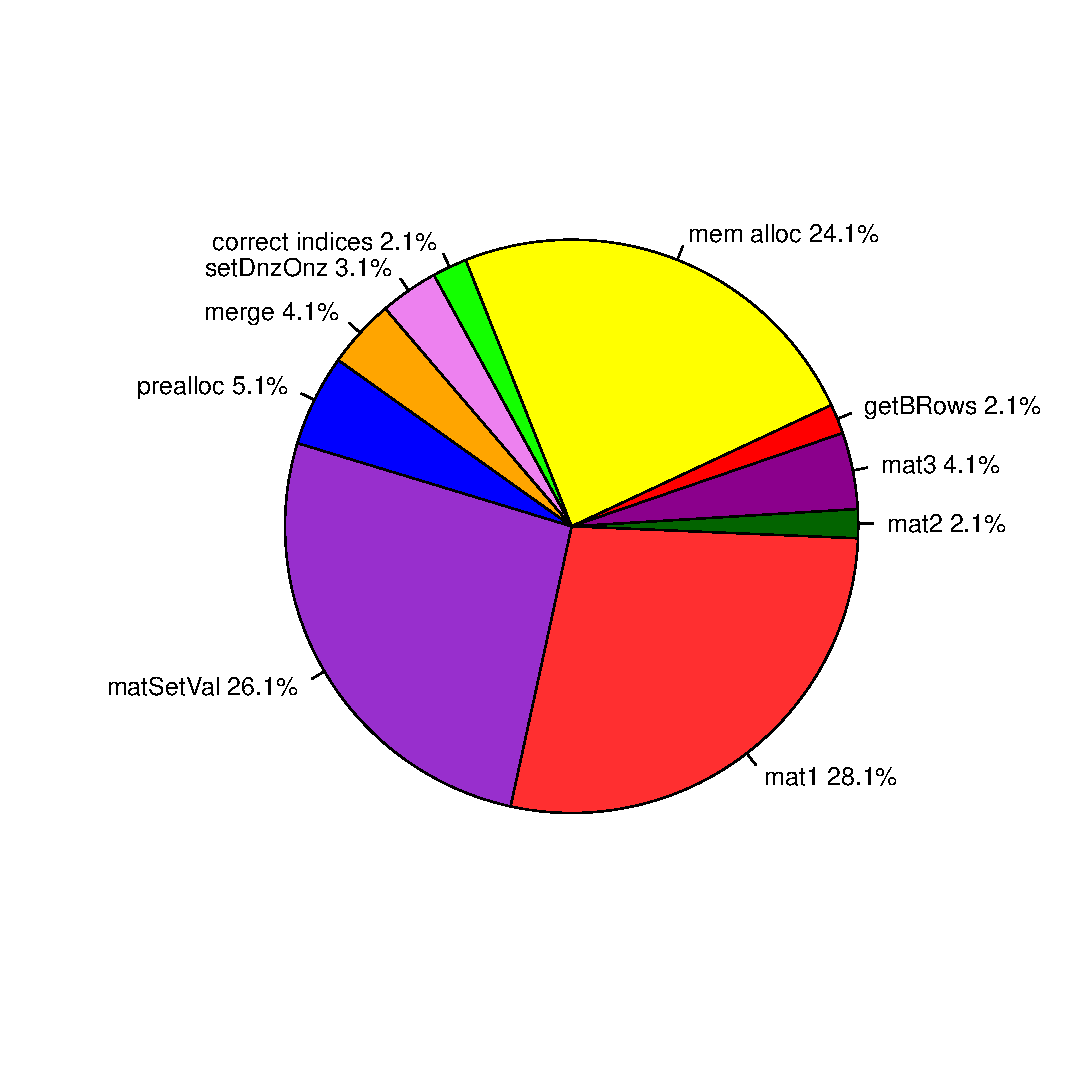
\includegraphics[width=1\textwidth, trim={0 3.cm 0 3cm},clip]{256cores_10240}
	\caption{MatMatMult for a $10240\times 10240$ grid, 256 cores, and a 2d, 13-point stencil.} 
	\label{fig:pie_256_10240}
\end{figure}

The reason why $A_{\textrm{loc, diag~}} B_{\textrm{loc, off}}$ (Mat2) is much faster than $A_{\textrm{loc, off~}} B_{\textrm{nonloc}}$ (Mat3), is that the result matrix for Mat3 is much bigger than the one for Mat2. Their sizes are $N/p \times N/p$ for Mat2 and $(N-N/p) \times (N-N/p)$ for Mat3, with a global matrix size $N\times N$ and $p\geq2$ processes. The higher the number of processes is, the higher is this difference.

With more than a quarter of the total time, the matSetValue routine needs much more time than one might expect. Also, the memory allocations need around a quarter of the total time. 

What is also very interesting here is the fact that only 2.1\% of the time is spent on getting non-local rows of $B$. That means if this function was to be implemented in an asynchronous way, i.e. the program does not wait with local multiplications until all non-local rows are retrieved, the multiplication could only be 2.1\% faster, for this setup. 

Other operations like merging the rows and preallocation only need around 15\% of total time.



\subsubsection*{5120 $\times$ 5120, 256 cores}
If the size of the grid is reduced from $10240 \times 10240$ to $5120 \times 5120$ while all other options stay the same, the results from Fig.~\ref{fig:pie_256_5120} are obtained. There are a few things that changed considerably: 

First, the share for time spent on getting the non-local rows of $B$ almost doubled (from 2.1\% to 4.1\%). This can be explained with Fig.~\ref{fig:large_small}: The boundary nodes of the local part of a grid are connected to non-local grid points. When the number of boundary grid points halves, the number of non-local rows that have to be retrieved also halves, while the total number of grid points decreases by a factor 4. That means the time spent on calculations decreases by a factor 4, while the time spent on retrieving non-local rows decreases by a factor 2. In combination, getBRows gets a slice of pie that is twice the size of before. 

The second share that changed a lot is the one for preallocation. This cannot be explained with the very nondeterministic behavior of the preallocation routines in PETSc (the time spent on this routines varies a lot), because the median of various measurements was taken. 

Except for these two sections (getBRows and preallocation), the relative amounts of time spent on the other sections stays almost the same compared to the previous experiment.

\begin{figure}[tbp]
	\centering
	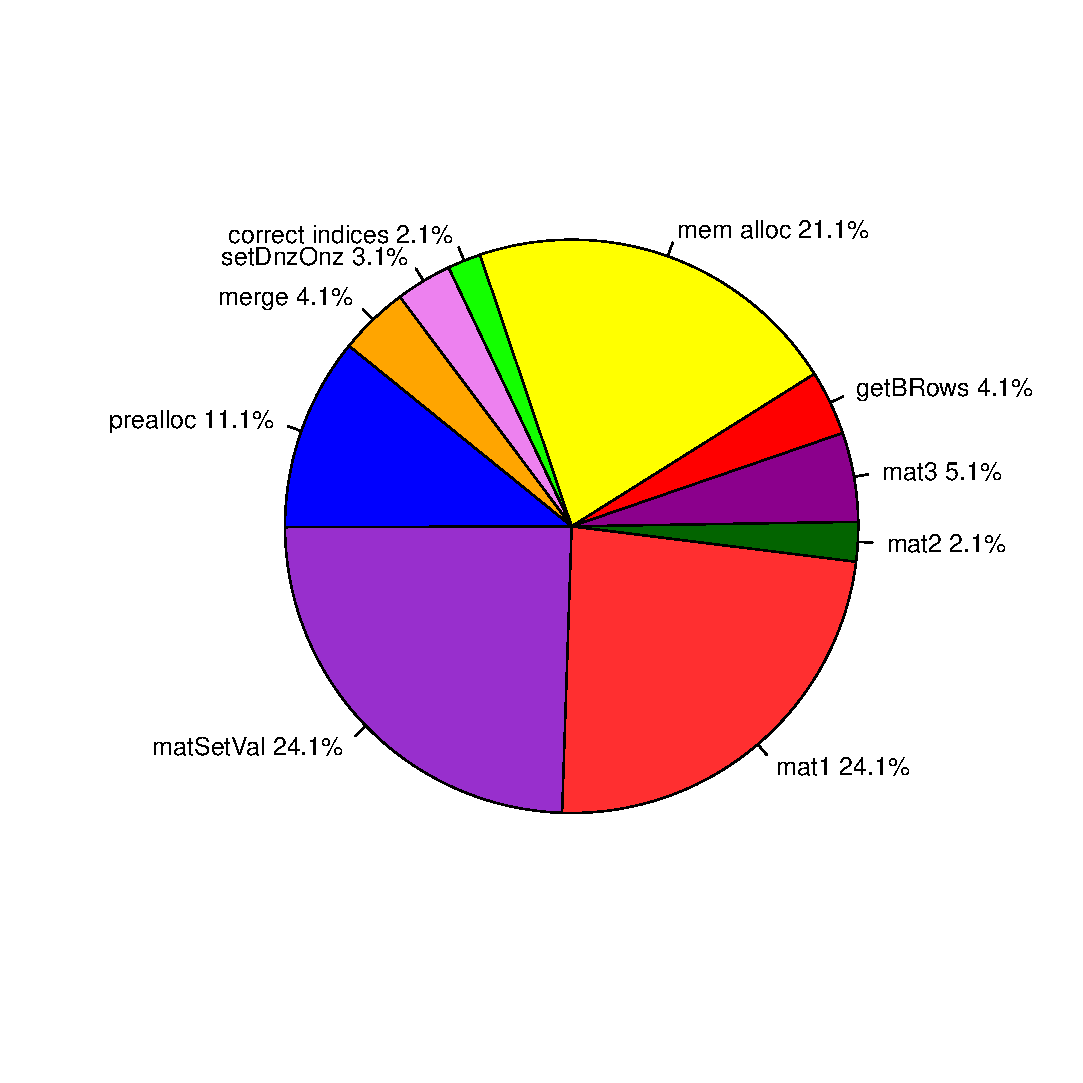
\includegraphics[width=1\textwidth, trim={0 3.cm 0 3cm},clip]{256cores_5120}
	\caption{MatMatMult for a $5120 \times 5120$ grid, 256 cores, and a 2d, 13-point stencil. Compared to the previous case (Fig.~\ref{fig:pie_256_10240}), the preallocation and the \textit{getBRows} operation changed a lot.} 
	\label{fig:pie_256_5120}
\end{figure}
\begin{figure}[tbp]
	\centering


	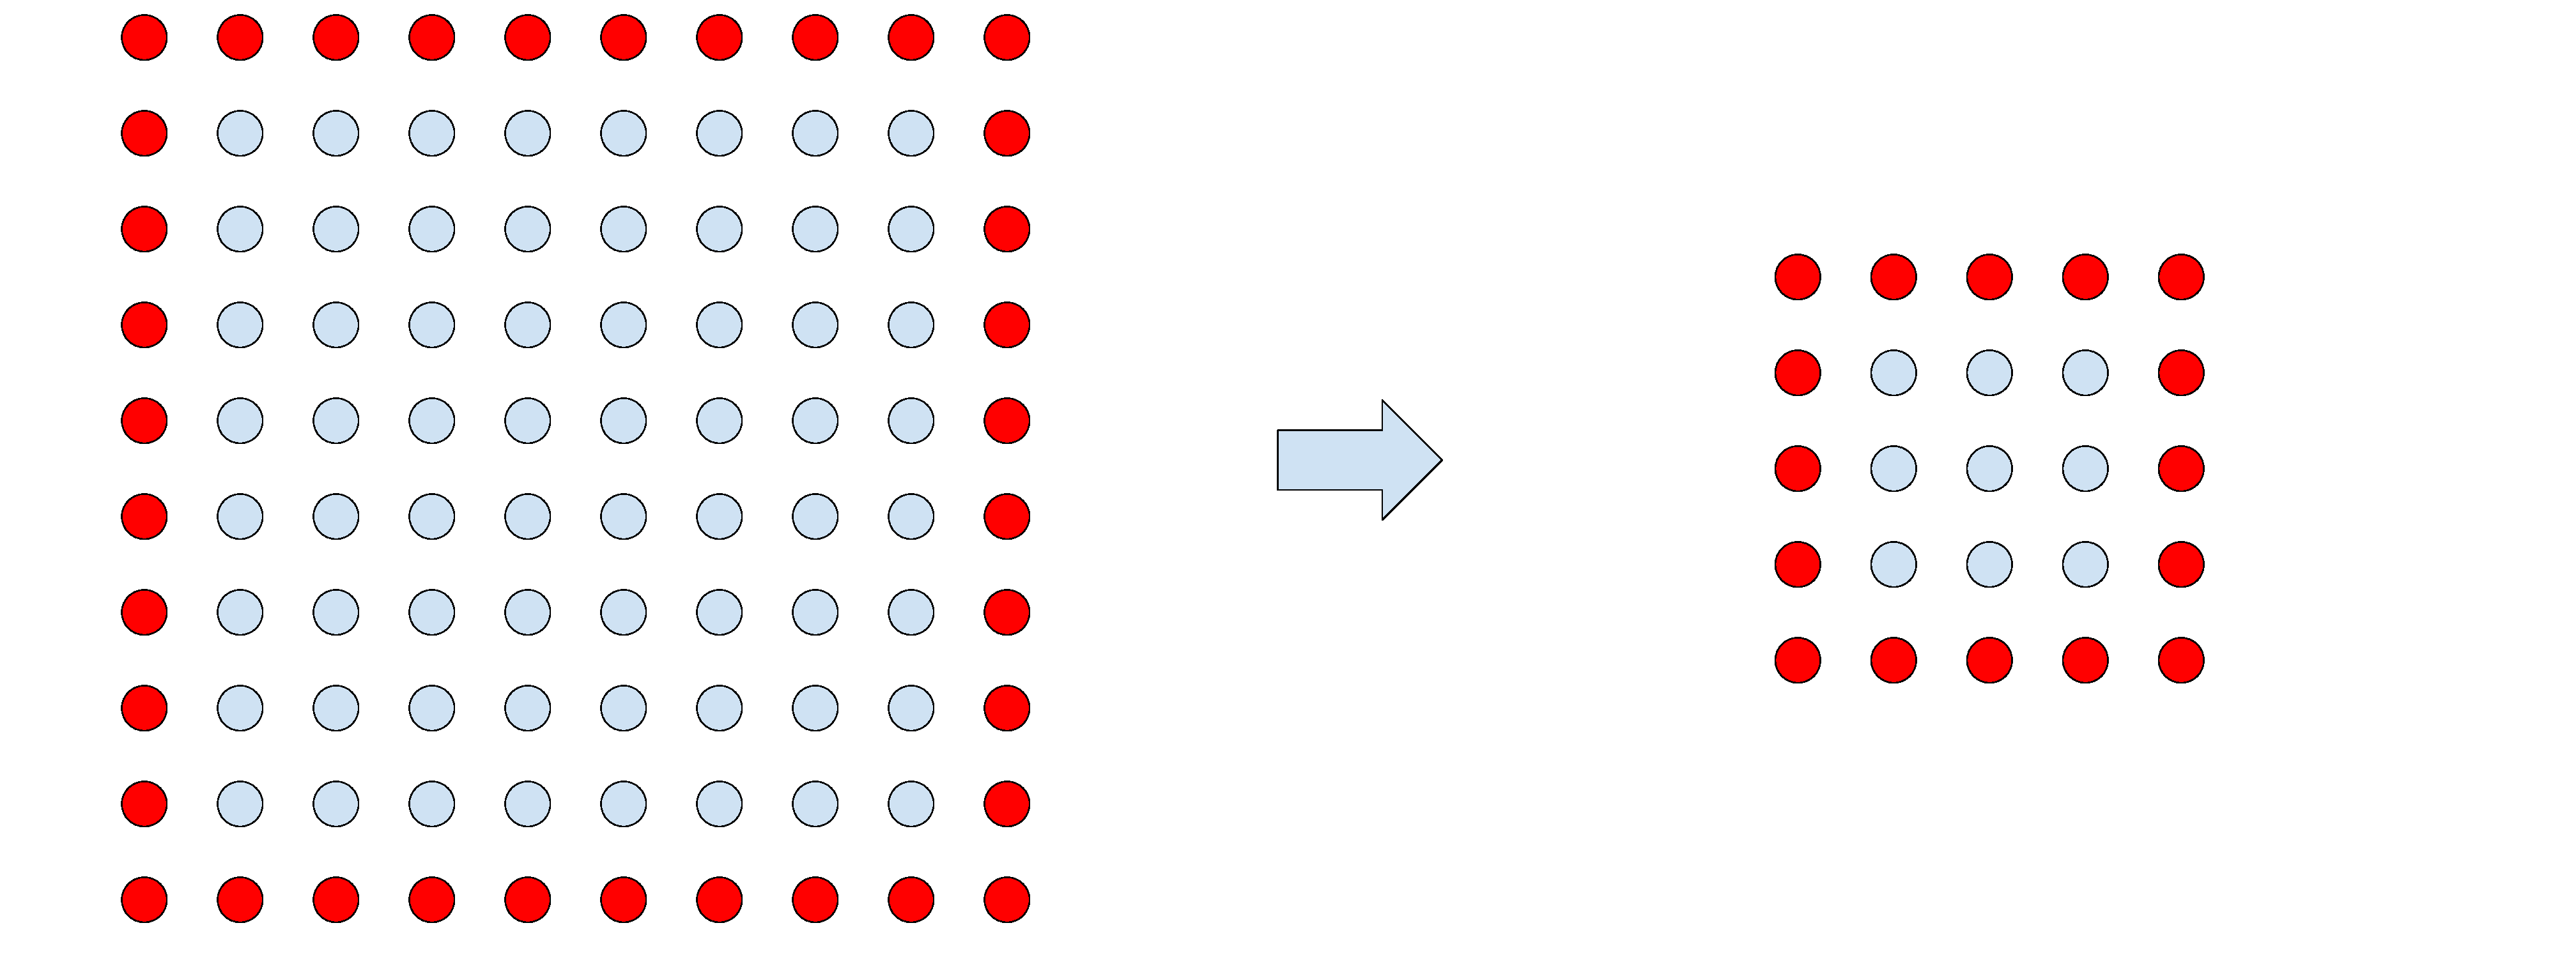
\includegraphics[width=1\textwidth]{4_large_small}
	\caption{The boundary nodes of the local part of a grid are connected to non-local grid points. When the number of boundary grid points halves, also the number of non-local rows that have to be retrieved halves, while the total number of grid points decreases by a factor 4.} 
	\label{fig:large_small}
\end{figure}

\subsubsection*{5120 $\times$ 5120, 16 cores}
For this experiment, the grid size stays the same, but only a 16th of the number of processor cores is used now. This leads to various big changes in our pie chart, which can be seen in Fig.~\ref{fig:pie_16_5120}. In order to explain these changes, it is useful to recall that the sizes of the result matrix are $N/p \times N/p$ for Mat2 and $(N-N/p) \times (N-N/p)$ for Mat3.

\begin{figure}[tbp]
	\centering
	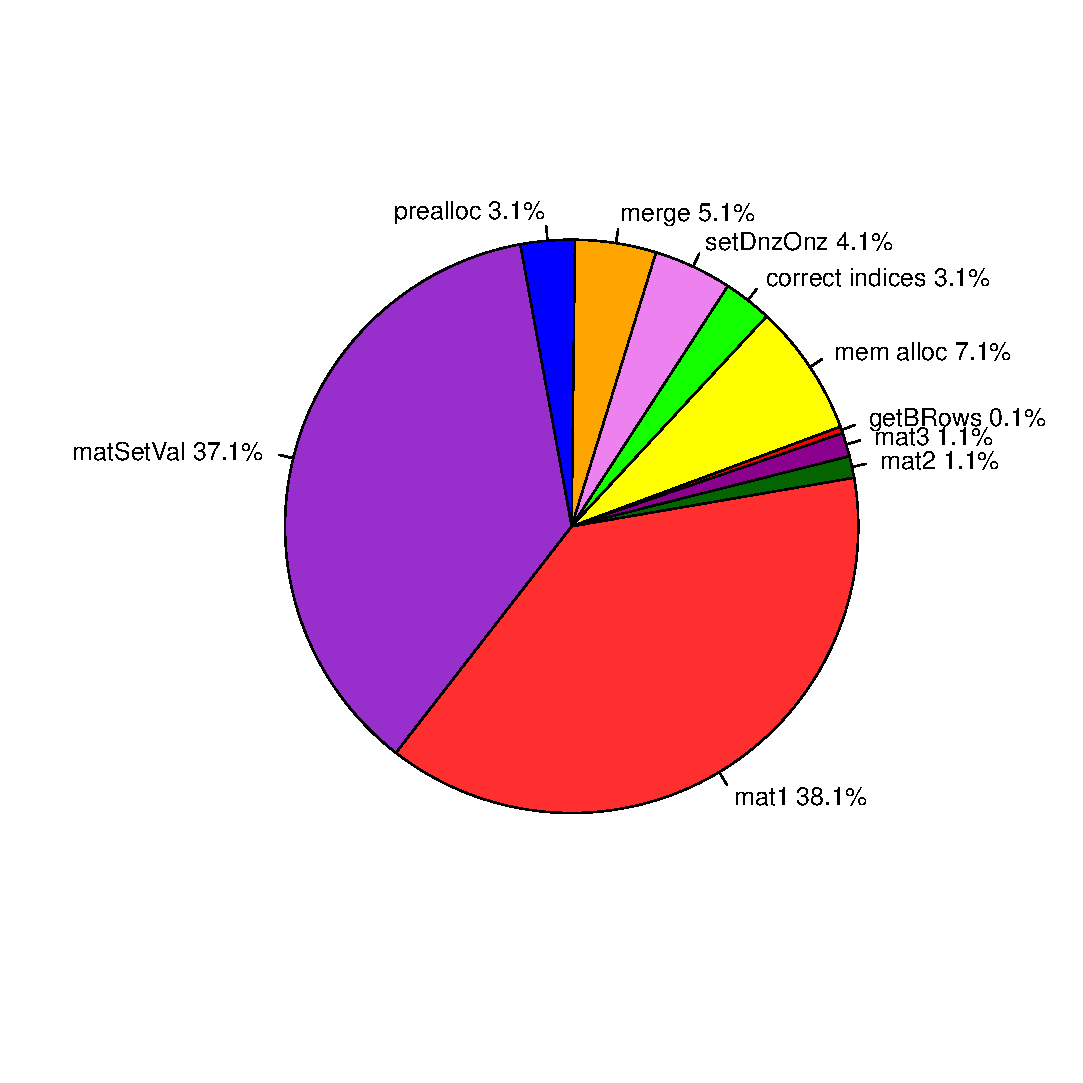
\includegraphics[width=1\textwidth, trim={0 3.5cm 0 3cm},clip]{16cores_5120}
	\caption{MatMatMult for a $5120 \times 5120$ grid, 16 cores, and a 2d, 13-point stencil} 
	\label{fig:pie_16_5120}
\end{figure}

Decreasing the number of processes yields a much bigger result matrix for Mat2 and a smaller one for Mat3. Therefore, Mat3 does not need so much time anymore; instead it needs as much time as Mat2. Also, the total number of off-diagonal elements decreases a lot because the diagonal blocks become much bigger. Hence, the time spent on Mat2 and Mat3 is much smaller now.

Next, we note that the time spent on retrieving the non-local rows of $B$ diminishes to 0.1\%. This is another result of the diagonal blocks being much bigger now, and it yields much fewer non-local elements of $B$.

Another share that decreases a lot (by a factor 3) is the time spent on memory allocations. Since the number of columns in the matrix stays the same, roughly the same amount of memory has to be allocated, so the absolute time spent on memory allocations stays almost the same. However, the multiplication takes much longer with 16 instead of 256 processes, so this share decreases a lot. 

The last share that decreased considerably (by a factor 3.5) is the one for the preallocation. The explanation is the same as for prior memory allocations: The total time stays roughly the same, while overall execution time increases very much. Also, the time spent on memory allocations is inherently quite nondeterministic, since the operating system may or may not have adequate free memory to assign at the moment of the request.

All mentioned decreases lead to a substantial increase of the time spent on matSetVal and on the multiplication $A_{\textrm{loc, diag~}} B_{\textrm{loc, diag}}$. The slices of pie for mat1 and matSetVal are both around 60\% bigger than before.

\subsubsection*{190 $\times$ 190 $\times$ 190, 32 cores}
The same experiment was done with a 3d system and a very big stencil. The system was of size $190 \times 190 \times 190$, the 3d, 27-point stencil was used and 32 cores were employed. The results fit in the picture that we have already got from the last experiment (see Fig.~\ref{fig:pie_32_190}): Since only a relatively low number of cores was used, the shares of Mat2 and Mat3 do not differ very much (Mat2 would be much faster than Mat3 for a high number of cores) and these shares are much smaller than the one of Mat1, but still bigger than they would be with a smaller stencil. 

\begin{figure}[tbp]
	\centering
	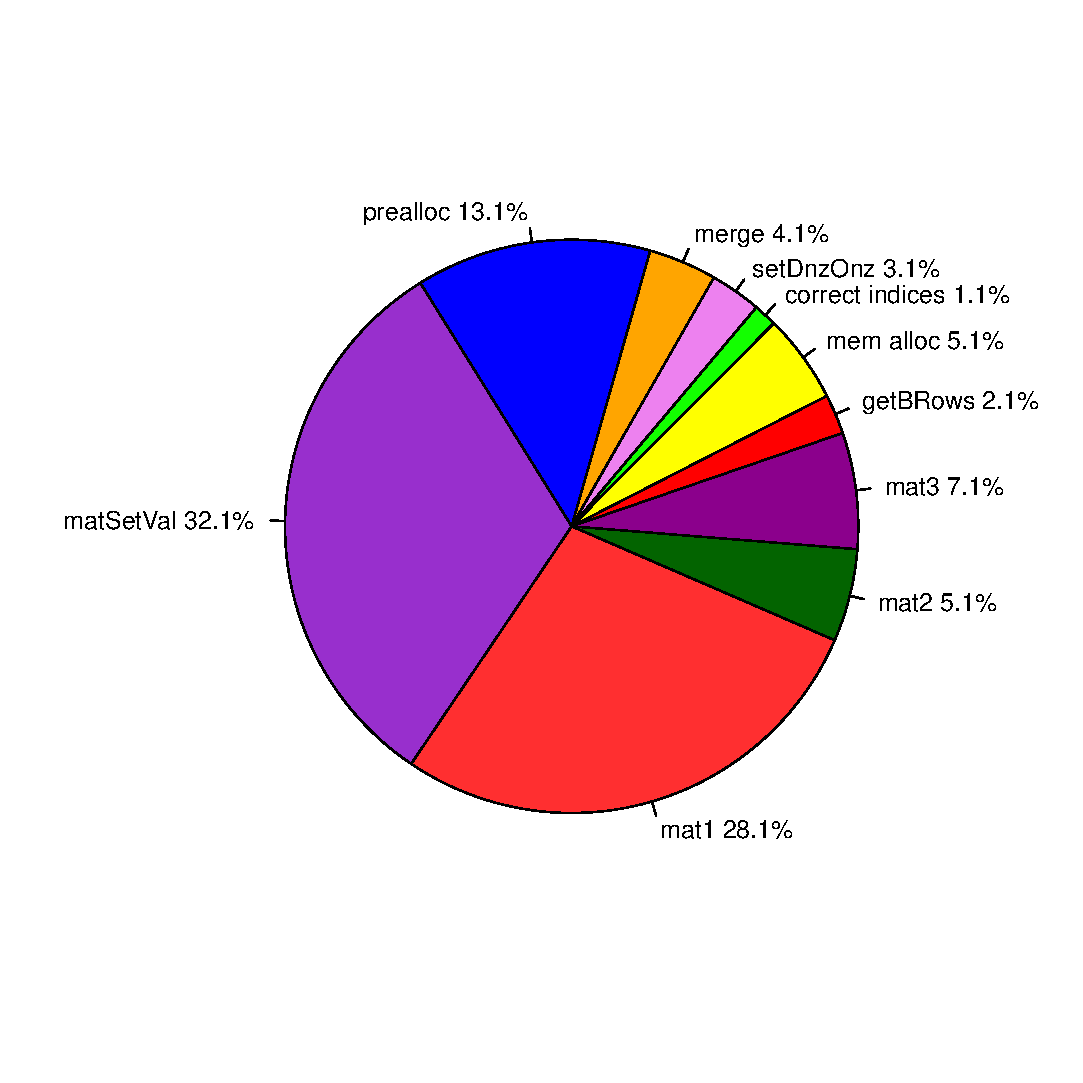
\includegraphics[width=1\textwidth, trim={0 3.5cm 0 3cm},clip]{32cores_190}
	\caption{MatMatMult for a $190 \times 190 \times 190$ grid, 32 cores and a 3d, 27-point stencil} 
	\label{fig:pie_32_190}
\end{figure}

\subsubsection*{Comparison of MatSetVal in different MatMatMult implementations}

Since the MatSetVal operation needs much more time than expected in the \textit{sequential MPI} implementation (sometimes more than a third of the total execution time), its duration was compared to the one of the \textit{nonscalable} implementation. The results can be seen in Fig.~\ref{fig:setvalues}. It became clear that the {MatSetVal} operation is always faster in the \textit{nonscalable} implementation, even though the same matrix values are set. The \textit{nonscalable} implementation only needs between 42\% and 77\% percent of the time the \textit{sequential MPI} implementation needs for setting the values of the matrix. 

However, the result of 42\% was obtained with an extremely small matrix. For bigger (and more relevant) matrices, still around 7-10\% of the time spent on the symbolic calculation could be saved if we assume that a third of time was spent on {MatSetVal} and the {MatSetVal} performance of the {nonscalable} implementation can be reached.  Therefore, this behavior still has to be analyzed further.


\begin{figure}[tbp]
	\centering
	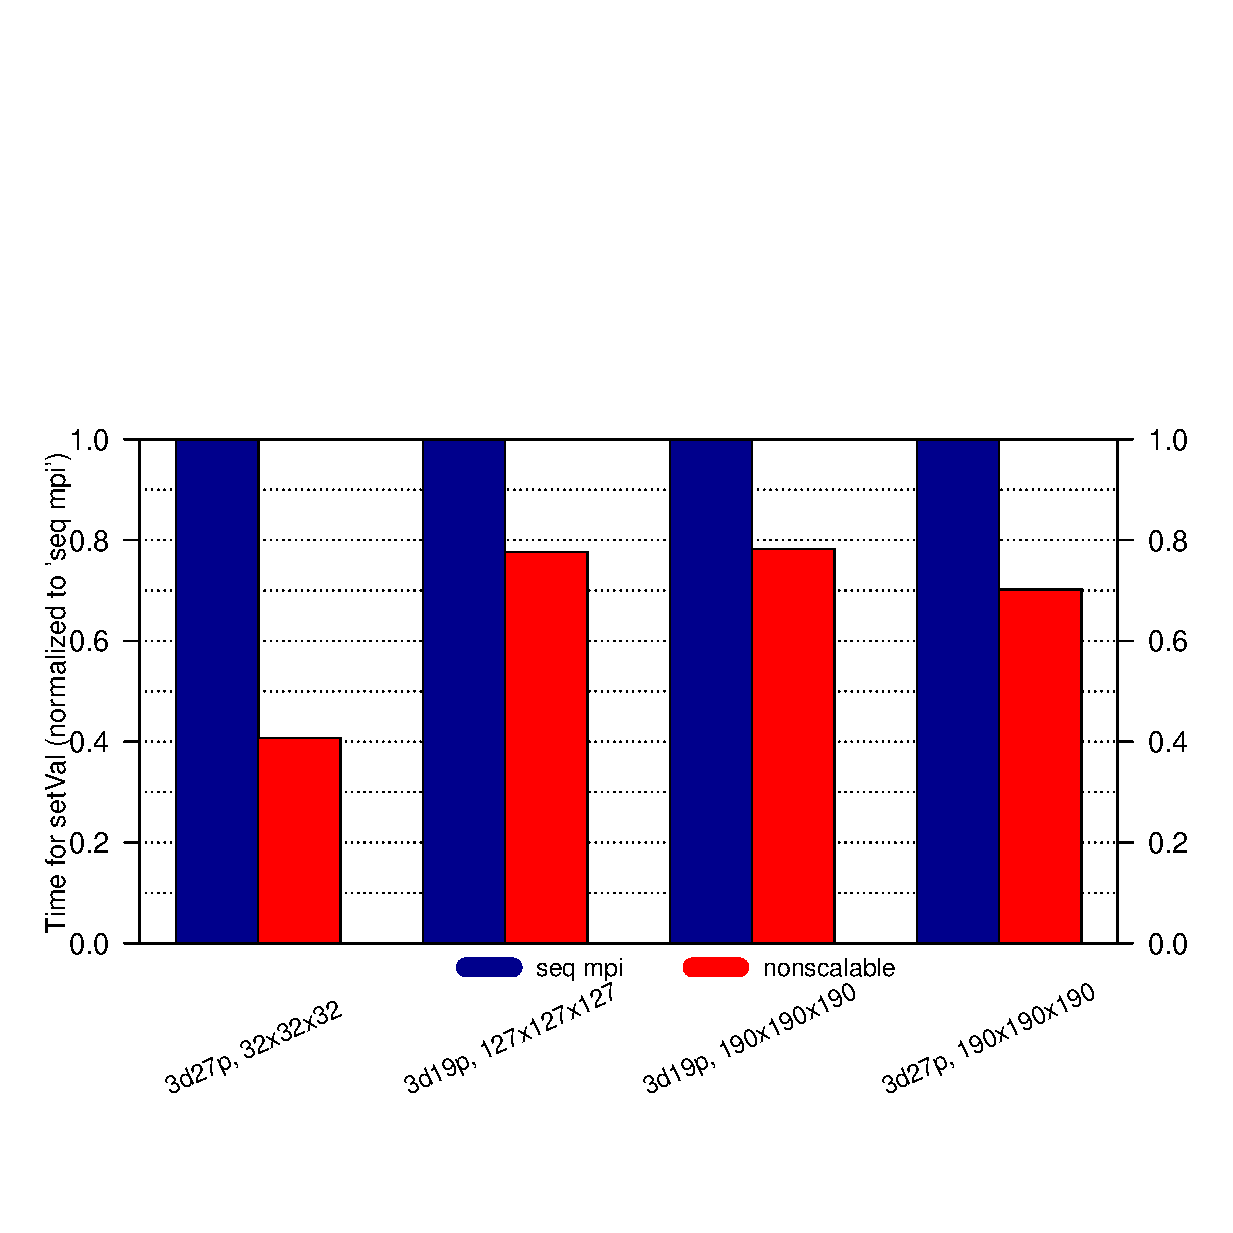
\includegraphics[width=1\textwidth, trim={0 2cm 0 7cm},clip]{setvalues}
	\caption{Normalized time for the \textit{setVal} operation. This is the step where the results of the symbolic calculation are written to the matrix.} 
	\label{fig:setvalues}
\end{figure}

\subsubsection*{Conclusion of this section}
Overall, these pie charts show that the biggest amount of time is usually spent on the sequential matrix multiplication $A_{\textrm{loc, diag~}} B_{\textrm{loc, diag}}$ and on the matSetValue routine, so any further optimizations here are of great value. The multiplication has already been attacked by analyzing the sequential matrix multiplication and choosing the fastest implementation, but of course there is still plenty of space for further optimizations. For matSetVal, the results show a high potential for obtaining better performance through optimizations.


\subsection{Time Ratio: Symbolic Calculation to Total Time}
Similar to the sequential case, the ratio of time spent on the symbolic calculation to the overall time spent on matrix multiplication was analyzed. For that, 256 MPI-ranks were employed. The small grids had a global size of $500\times 500$ (local size: $32\times 32$) for the 2d stencils and $30\times 30 \times 30$ (local size: $5\times 5 \times 5$) for the 3d stencil. The large grids had a global size of $14000\times 14000$ (local size: $875 \times 875$) for the 2d stencils and $300 \times 300 \times 300$ (local size: $47\times 47 \times 47$) for the 3d stencil. 

As can be seen in Fig.~\ref{fig:mpi_symnum}, the ratio of time spent on the symbolic calculation to the overall time is around 90\% for all stencils. For small grids this ratio is even bigger than for large grids. That means spending time on the optimization of the numeric stage is unlikely to be of great use. Instead, all further optimizations should be focused on the symbolic stage. 

\begin{figure}[tbp]
	\centering
	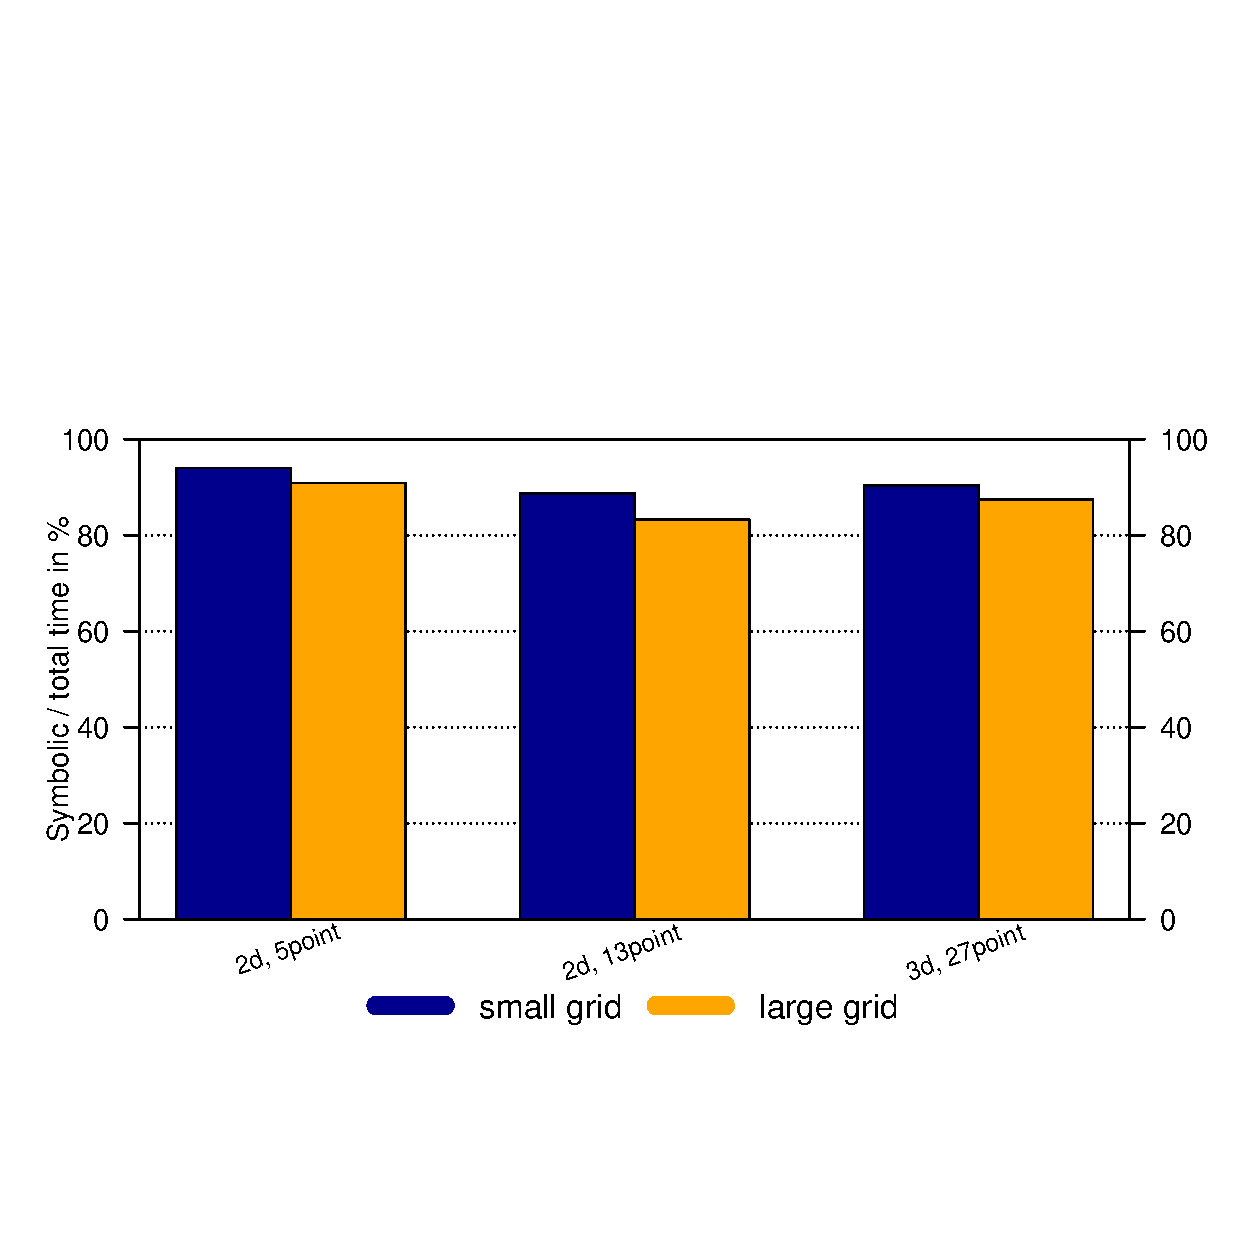
\includegraphics[width=1\textwidth, trim={0 3.cm 0 7cm},clip]{mpi_symnum}
	\caption{Percentage of time spent on the symbolic stage of the matrix multiplication of the total execution time for the \textit{sequential MPI} implementation. The rest to 100\% is spent on the numeric stage.} 
	\label{fig:mpi_symnum}
\end{figure}

\section{Stages of Multigrid}
Next the times for different stages of the multigrid solvers GAMG and Hypre were analyzed. 
GAMG is the multigrid preconditioner that is implemented in PETSc and Hypre is an external package \cite{hypre-web-page}. 

The GAMG multigrid implementation is based on the hierarchy that can be seen in Fig.~\ref{fig:multigrid_hierarchy_gamg}. This figure also shows the percentage of time that is spent on each stage of the implementation, when a single V-cycle is performed. The grid had a global size of $512\times 512$ and 256 processes were used.

All computational work is done in the KSPSolve phase. This phase is divided into a setup phase (PCSetUp) and a phase where the preconditioner is applied (PCApply). In the setup phase, the entire multigrid hierarchy is build up. This takes around 91\% of the time spent on KSPSolve. In this phase, the coarse grid is created algebraically (PCGAMGCoarse\_AGG, 37.3\% of the setup phase), and the fine grid operators are created with the Galerkin product
\begin{equation}
L_H = I_h^H L_h I_H^h = (I_H^h)^T L_h I_H^h
\end{equation}
as described in Chapter~2. For that, regular matrix-matrix multiplications (MatMatMult, 14.7\%) and matrix multiplications with the transposed matrix (13.6\%) are used. The symbolic stage takes a similar share of the matrix multiplication as in previous experiments ($\approx 80\%)$.

\begin{figure}[tbp]
	\centering
	\hspace*{-7mm}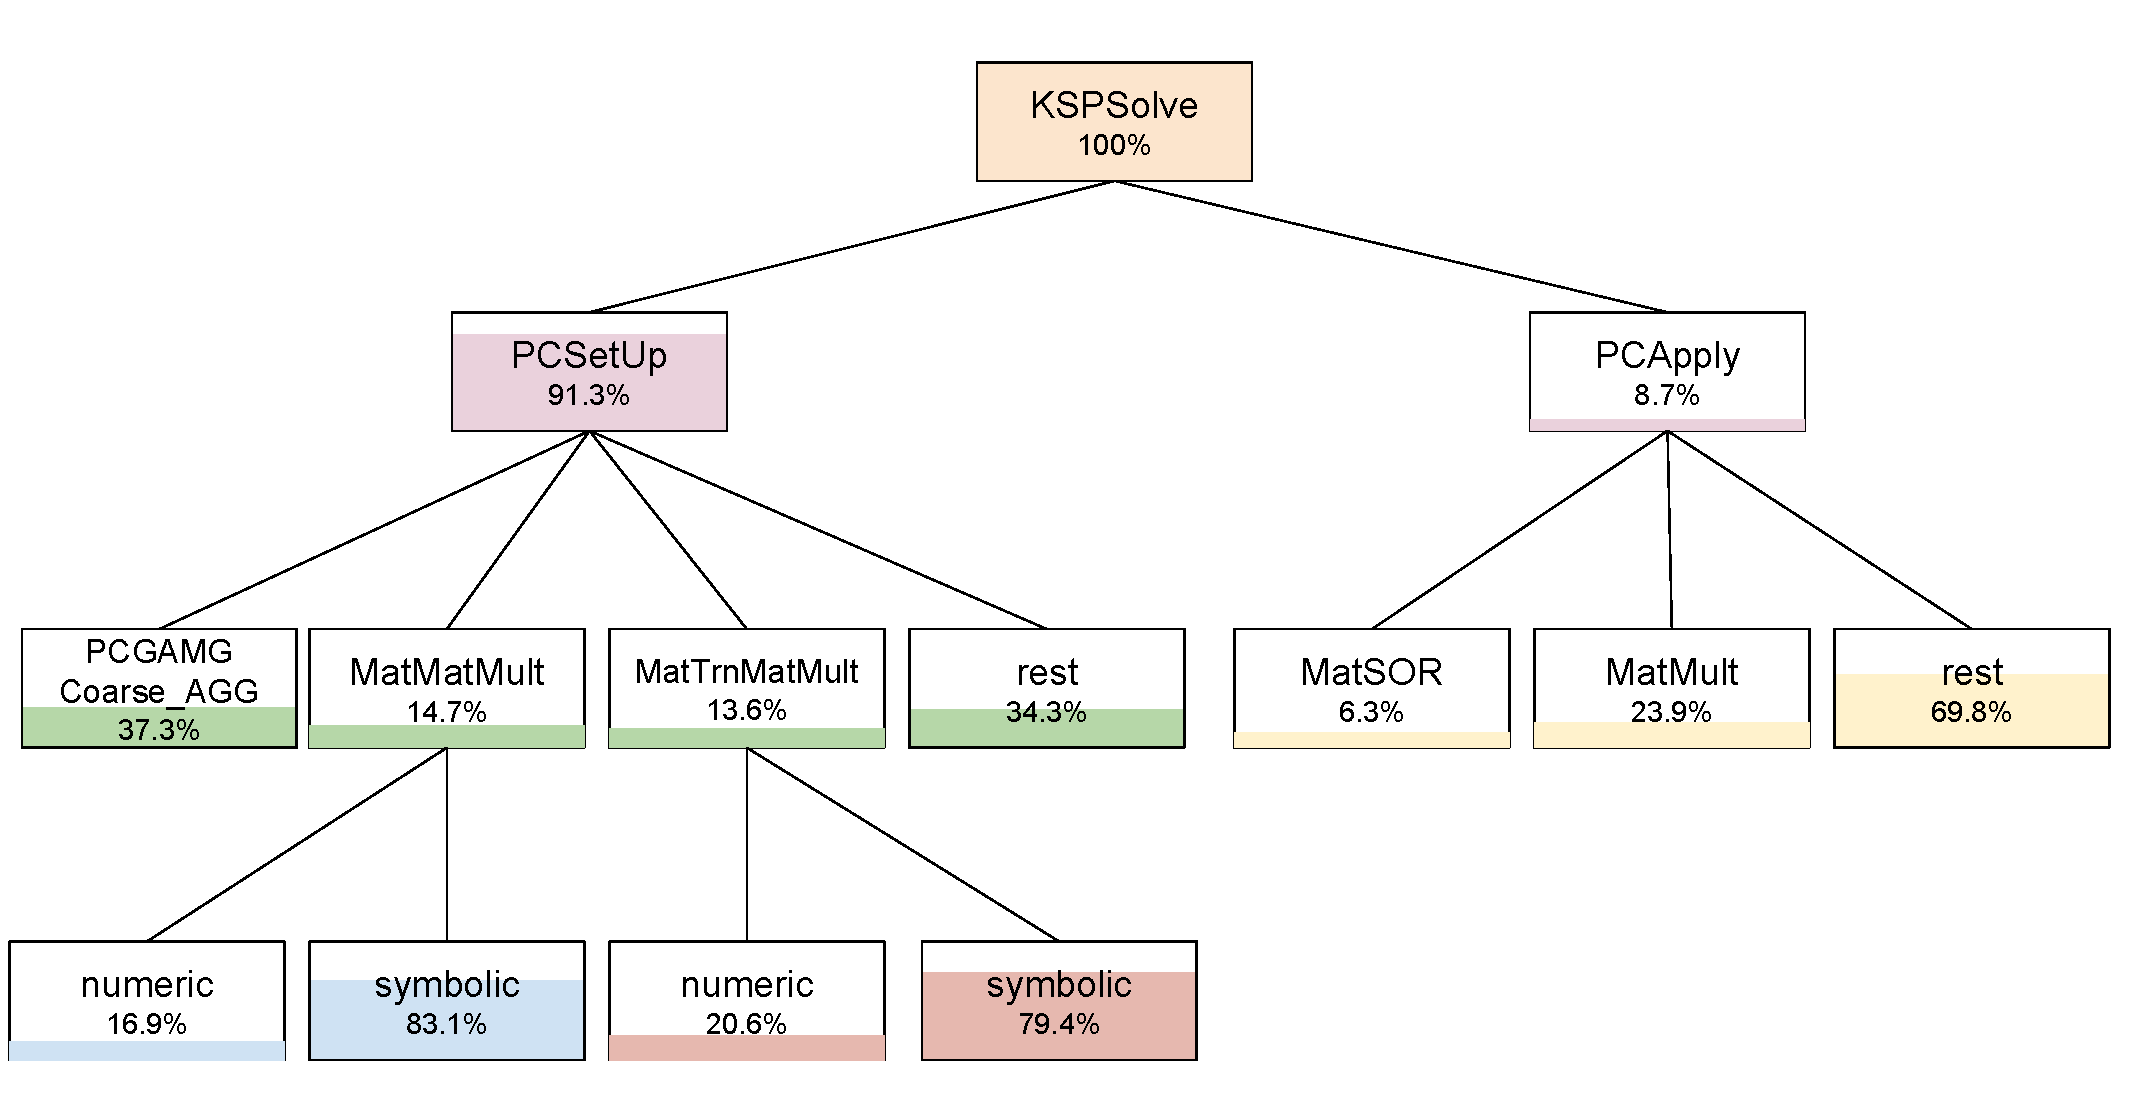
\includegraphics[width=1.1\textwidth]{Multigrid_hierarchy_GAMG}
	\caption{Multigrid stages in GAMG.} 
	\label{fig:multigrid_hierarchy_gamg}
\end{figure}

After the setup is complete, the preconditioner is applied with PCApply. That only takes around a tenth of the time that is spent on the setup phase, since only one iteration is performed here. When there are only a few iterations, PCApply is faster than PCSetUp, while it takes more time with many iterations. In a well-balanced solver, these operations should take roughly the same amount of time. 

PCApply basically comprises a MatMult and a MatSOR stage. MatSOR (Matrix successive over relaxation) is a Jacobi iteration with a relaxation parameter, so this is the step where the error smoothing is done. This only takes 6.3\% of the time for the PCApply stage. Other steps that are included within PCApply are a direct solve and bookkeeping operations.

Since Hypre is an external package, there is no such detailed output about different stages of this preconditioner. In Fig.~\ref{fig:multigrid_hierarchy_hypre}, the division of PCSetUp and PCApply is shown. Now, the share for the time spent on PCApply increased to around a third. That is due to a major change in the setup time: The setup in Hypre only needs around a ninth of the time the setup in GAMG needs. 

\begin{figure}[tbp]
	\centering
	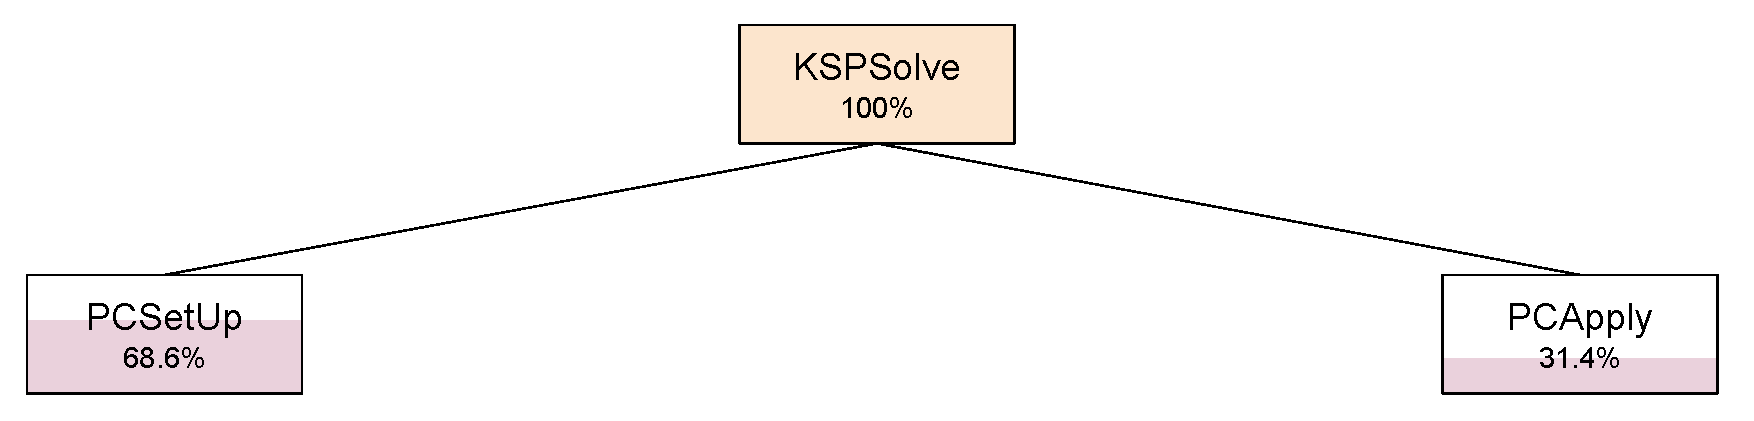
\includegraphics[width=1.\textwidth]{Multigrid_hierarchy_Hypre}
	\caption{Multigrid stages in Hypre.} 
	\label{fig:multigrid_hierarchy_hypre}
\end{figure}



\section{Strong and Weak Scaling Properties of Solvers}

In this section the strong scaling and weak scaling capabilities of different solvers are evaluated. Testing a program for its strong scaling capabilities means that there is a fixed problem size and the problem is solved by using different numbers of processes. Ideally, the time is inversely proportional to the number of processes used: $T \propto 1/\textit{\#processes}$. For weak scaling, the problem size per process is fixed and the program is executed with different numbers of processes, so the total problem size changes. Both scaling methods are illustrated in Fig.~\ref{fig:strong_weak_scaling}. 

However, the ideal results cannot be obtained because of relatively slow networks and latencies.



\begin{figure}[tb]
	\centering
\hspace*{-7mm}	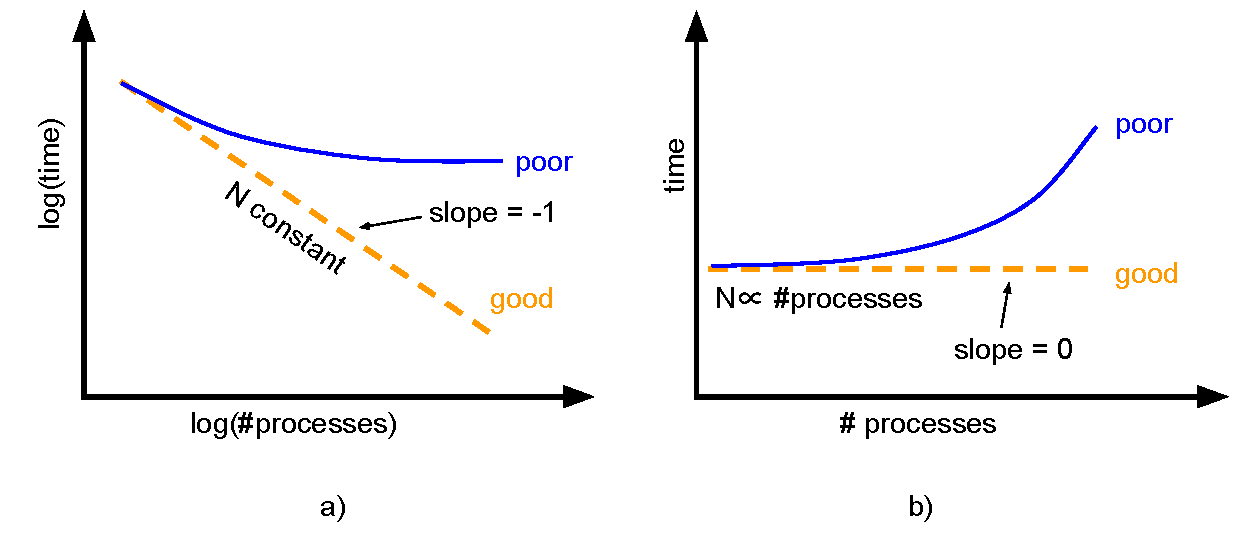
\includegraphics[width=1.\textwidth]{4_strong_weak_scaling}
	\caption{\textbf{a)} Strong scaling: The total problem size is fixed, so when the number of processes increases, the time to execute the program ideally decreases proportional to a $1/x$ curve. \textbf{b)} Weak scaling: Here the problem size per process is fixed, so ideally the execution time does not depend on the number of processes.}
	\label{fig:strong_weak_scaling}
\end{figure}


\subsection{Strong Scaling}


Strong scaling results were obtained for measuring the performance of different solvers for a linear system $Ax = b$ that arose from discretizing Poisson's equation. The iterative solvers for the system relied on an iteration method called Generalized minimal residual method (GMRES) \cite{saad1986gmres}, and also a direct solver, the LU decomposition, was used. All programs were only stopped when a specific accuracy of the result was reached. The following methods were tested:
\begin{itemize}
\item Jacobi preconditioner with GMRES,
\item No preconditioner, so only the GMRES method is used here,
\item GAMG, the multigrid solver that is implemented in PETSc,
\item HYPRE, multigrid solver from an external package,
\item Solving the system directly with the LU decomposition (no iterative method)
\end{itemize}


The solution of the hydrostatic equation was one of the experiments that were performed to determine the strong scaling properties of the different solvers (see Fig.~\ref{fig:res_ex2_strong_time}). Except for the direct method, all solvers show good scalability if there are many (more than ca. 16k) unknowns per rank. Especially  the Hypre \cite{hypre-web-page} preconditioner shows very impressive results as long as the local problem size is big enough. Only with very small local sizes, the slopes become flat for all preconditioners except Jacobi. However, the total computational work is much bigger with the Jacobi preconditioner, so the scalability is better while the overall performance is poor. This example proves that multigrid solvers like GAMG or Hypre perform much better than conventional methods. 


\begin{figure}[tb]
	\centering
	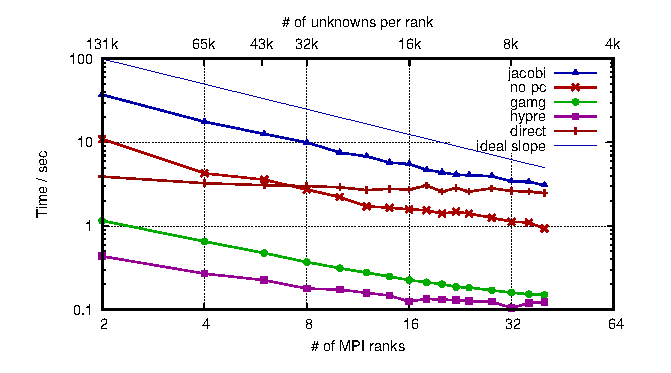
\includegraphics[width=0.99\textwidth]{ex2_times}
	\caption{Strong scaling: Solving a linear system $Au = x$ with $2^{18} = 262k$ global unknowns with different solvers until the results have converged.} 
	\label{fig:res_ex2_strong_time}
\end{figure}

The strong scaling properties of \textbf{another example} can be seen in Fig.~\ref{fig:res_ex48}, where the GAMG multigrid solver is used to solve a system $Au = b$ that arises from the nonlinear hydrostatic equation for ice flow. Here, the difference between using 4 MPI-ranks per node and using 16 MPI-ranks per node was observed. The total number of MPI-ranks was the same for both cases.

The results show that the difference between 4 and 16 ranks/node are rather small. The reason why the performances are so similar is that the performance is limited by latencies. These latencies are almost independent of the number of ranks per node. The small difference in favour of 16 ranks/node is due to the high computational work for each rank.

If less than ca. 15,000 unknowns are to be computed by each process (rank), the computing power of additional ranks cannot be fully exploited any more because the local matrices become very small and much data has to be transferred from one rank to another. For 500 MPI ranks, only around two thirds of the ideal performance can be reached. 


% ex48  (strong scaling)
\begin{figure}[tb]
	\centering
	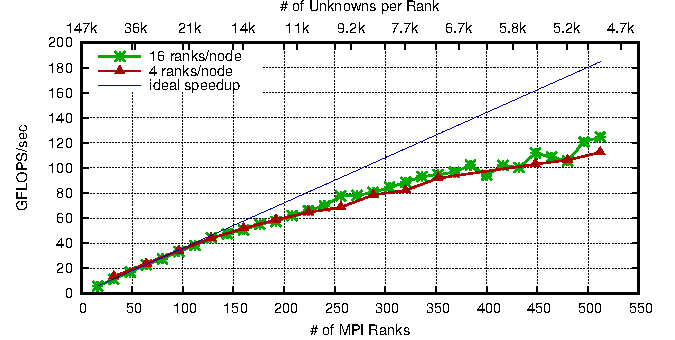
\includegraphics[width=0.99\textwidth]{ex48}
	\caption{Strong scaling: An example of the use of a GAMG solver that shows strong scaling effects. For less than ca. 15k unknowns per process, the computing power of additional ranks cannot be fully exploited any more. It can also be seen that 16 ranks/node is very often slightly faster than 4 ranks/node, when using the same total number of ranks.} 
	\label{fig:res_ex48}
\end{figure}


% ex2_strong

\subsection{Weak Scaling}

The weak scaling properties of different solvers were tested for both a limited number of iterations and an unlimited number of iterations. In order to quantify weak scalability, a factor $\alpha_{p \rightarrow q}$ is defined as $\alpha_{p \rightarrow q} = \frac{T_q}{T_p}$, with $T_x$ being the time to solve the problem with $x$ processes. For ideal weak scaling, this ratio is 1. 

\subsubsection*{Max. 50 iterations}

For this experiment, a system $Au = x$ with 262k unknowns per MPI rank was solved. This corresponds to a $512 \times 512$ local grid. A 2d, 5-point stencil was used and the calculation was stopped after 50 iterations in order to not take too much time. Hence, the results differ in accuracy for different solvers and the absolute time until 50 iterations were performed is not relevant. What is relevant, though, is the slope of each curve. The results are shown in Fig.~\ref{fig:ex2_weak_time}. 

A solver with good weak scaling properties, i.e. an execution time that does not depend much on the global problem size, \textit{seems to be} the Jacobi preconditioner. Here the performance per core only differs by a factor 2 when 1024 instead of 1 cores are used ($\alpha_{1 \rightarrow 1024} = 2$). Also, the other iterative solvers perform quite well:  $\alpha_{1 \rightarrow 1024}$ is around 4 if no preconditioner is used, around 8 for GAMG, and 10 for Hypre. 

On the other hand, solving the system directly with the LU factorization does not scale at all. The reason for that is quite simple; there is no parallel implementation for this direct solver in PETSc.

\begin{figure}[tb]
	\centering
	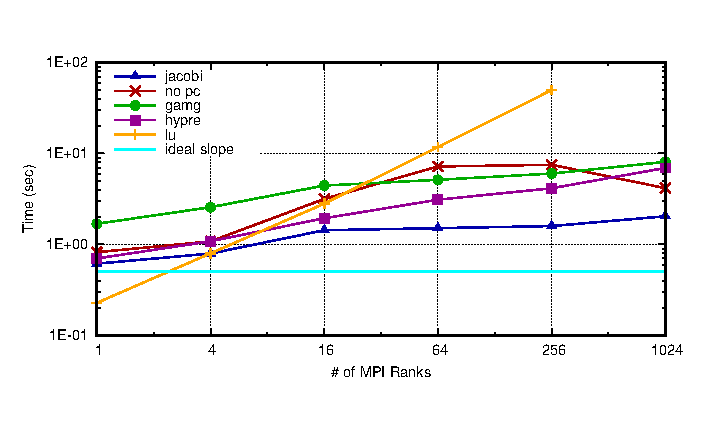
\includegraphics[width=0.99\textwidth]{ex2_weak_time}
	\caption{Weak scaling: Solving a linear system $Au = x$ with $2^{18} = 262k$ unknowns per process with different solvers. The calculations were stopped after 50 iterations.} 
	\label{fig:ex2_weak_time}
\end{figure}

\subsubsection*{Unlimited iterations}
The time until a specific accuracy of the result is reached can be seen in Fig.~\ref{fig:ex2_weak_nomaxit}. That means there is no maximum number of iterations. Now the local size of the system was reduced from $512\times 512$ to $128\times 128$ in order to not take too much time. The 2d, 5-point stencil stays the same.

The results about scalability that were obtained from the last experiment prove to be only partly true now: While $\alpha_{1 \rightarrow 1024}$ is the same for the multigrid solvers GAMG and Hypre ($\alpha_{1 \rightarrow 1024, \textrm{GAMG}} =8$ and $\alpha_{1 \rightarrow 1024, \textrm{Hypre}} =10$), this factor is very different for the Jacobi preconditioner and for solving the system without preconditioner: For Jacobi, $\alpha_{1 \rightarrow 1024}$ changed from 2 to 30 and for no preconditioner from 4 to 100. The reason for that is that for these solvers, the number of iterations changes considerably when the global problem size changes. This shows another advantage of multigrid methods: The number of necessary iterations is almost independent of the global problem size.

In order to conclude this section, we take a look at the absolute numbers rather than scalability ratios. The Hypre multigrid method shows the best results (except for one outlier) as it needs only a few dozens of $\mu s$ to solve a local grid of size $512\times 512$. GAMG is  10-15\% slower than Hypre and the other tested solvers are not competitive.

\begin{figure}[tb]
	\centering
	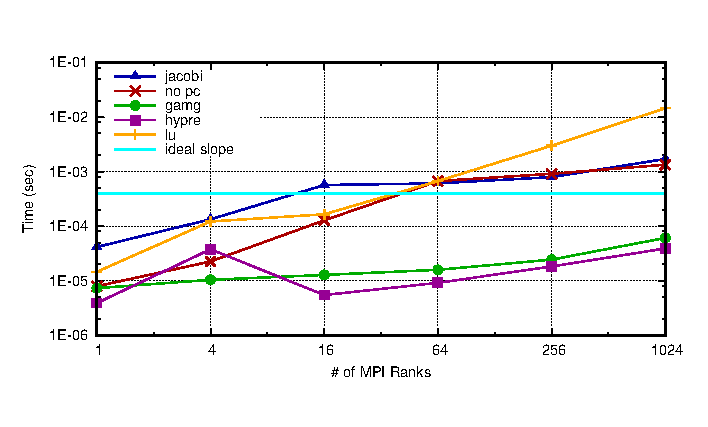
\includegraphics[width=0.99\textwidth]{ex2_weak_nomaxit}
	\caption{Weak scaling: Solving a linear system $Au = x$ with $2^{14} = 16384$ unknowns per process with different solvers. } 
	\label{fig:ex2_weak_nomaxit}
\end{figure}
